% SIAM Shared Information Template
% This is information that is shared between the main document and any
% supplement. If no supplement is required, then this information can
% be included directly in the main document.
%Keeping in mind the observations from previous \Cref{Sec:motivation}, one can observe that it would be best to maintain the nonzeros of matrix close to the diagonal.

%%Improving data locality for sparse matrix computations
%%like \acrshort{SpMV} often requires bandwidth reduction via
%%pre-processing algorithms such
%%as \acrfull{RCM} \cite{RCM,RCM_Sparse_computation}. In RACE, we thus
%%start with a bandwidth reduction approach and then apply a
%%locality-conserving coloring scheme, recursively if necessary to
%%obtain a sufficient level of parallelism. The recursion is designed
%%to avoid global synchronization between threads.
%Here, we aim to develop a method that does not distort this ideal permutations to a large extent and at the same time resolves \DK dependencies. 
Our advanced coloring algorithm is based on three steps:
\begin{enumerate}
	\item level construction,
	\item \DK coloring,
	\item load balancing.
\end{enumerate}
In the first step we apply a bandwidth reduction algorithm
including level construction and matrix reordering. We then use the
information from the level construction step to form subsets of levels
which allow for hardware efficient \DK coloring of the graph. Finally
we present a concept to ensure load balancing between threads. These steps
are applied recursively if required.


%The method is strongly coupled to the hardware underneath and exploits only the parallelism as required by the hardware. If at the end of all these four steps one does not achieve sufficient parallelism, all the steps are recursively applied to selected sub-graphs of the matrix until sufficient parallelism is attained. Due to this recursive nature of our coloring method we cal it as ``\RACfullNoSpace" (\RAC).

To illustrate the method we choose a
simple matrix which is associated with an artificially constructed
two-dimensional stencil as shown in \Cref{fig:2d-7pt-a}. The
corresponding sparsity pattern and the graph of the matrix are shown
in \Cref{fig:2d-7pt-b,fig:2d-7pt-c} respectively.
\begin{figure}[t]
	\centering
	\subfloat[\Stex]{\label{fig:2d-7pt-a}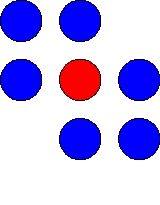
\includegraphics[width=0.17\textwidth , height=0.13\textheight]{pics/2d-7pt/stencil.pdf}}
	\hspace{0.8em}
	\subfloat[Sparsity
	 pattern]{\label{fig:2d-7pt-b}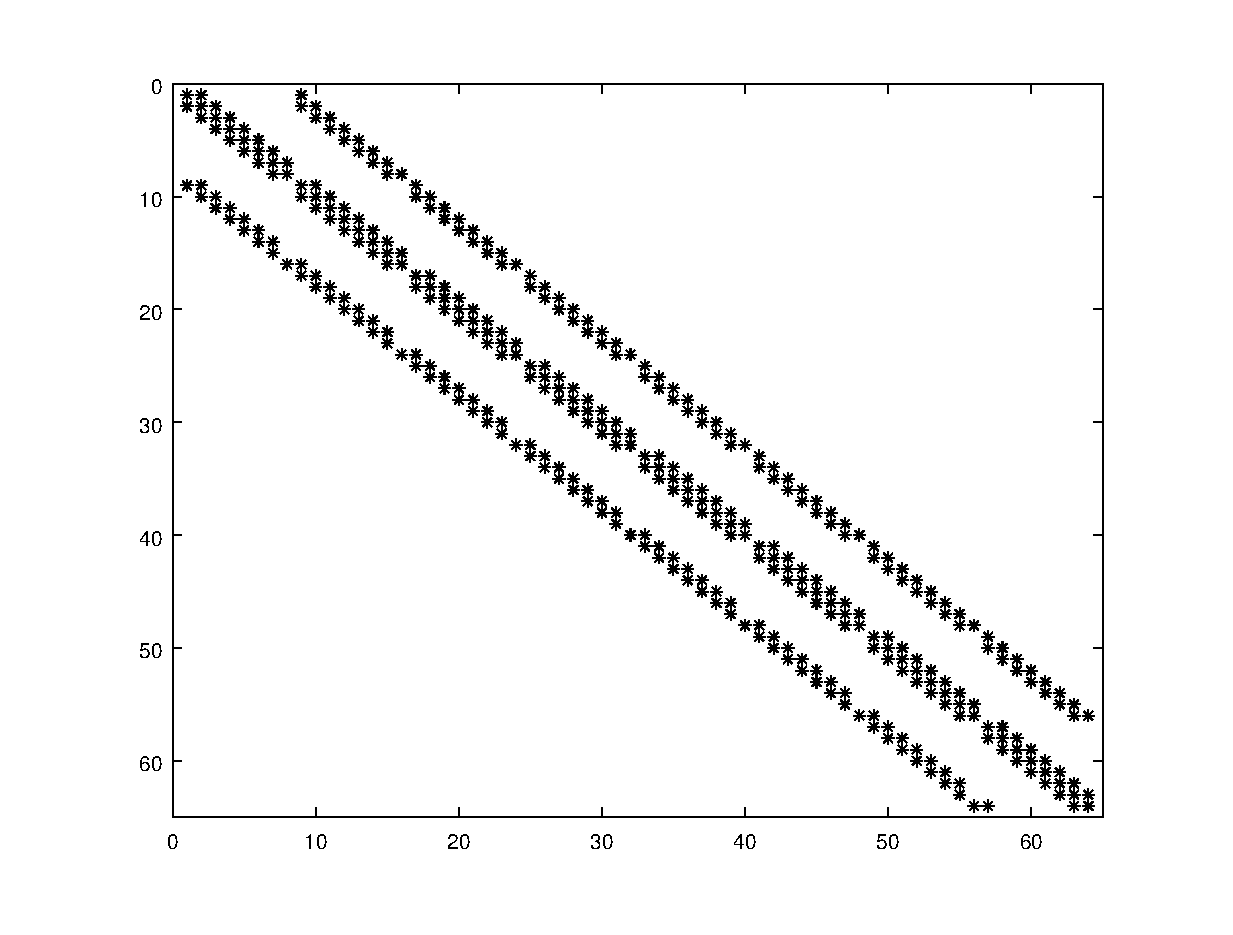
\includegraphics[width=0.38\textwidth , height=0.19\textheight]{pics/2d-7pt/2d_7pt_bw.eps}}
	\hspace{1em}
	\subfloat[Graph]{\label{fig:2d-7pt-c}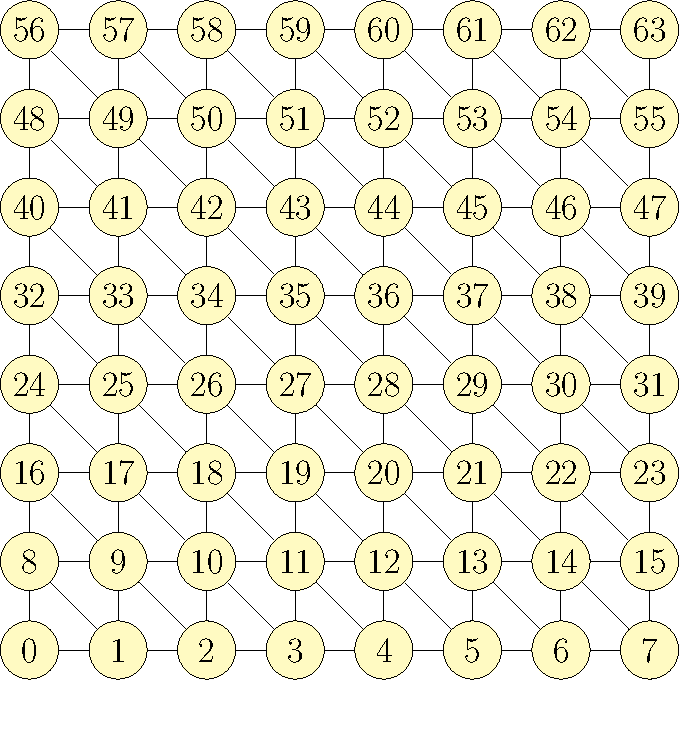
\includegraphics[width=0.3\textwidth , height=0.18\textheight]{pics/2d-7pt/stencil_2d_7pt.pdf}}
	\caption{\sref{fig:2d-7pt-a} Structure of an artificially designed stencil,
	\sref{fig:2d-7pt-b} corresponding sparsity pattern of its matrix
	representation on an $8\times 8$ lattice with Dirichlet
	boundary conditions, and \sref{fig:2d-7pt-c} the graph representation of the
	matrix. The stencil
	structure was chosen for illustration purposes and does not
	represent any specific application scenario.}
	\label{fig:2d-7pt}
\end{figure}

\subsection*{Definitions}
We need the following definitions from graph theory:
\begin{itemize}
	\item \textbf{Graph: } $G = (V,E)$ represents a graph, with $V(G)$
              denoting its set of vertices and $E(G)$ denoting its edges. Note that
              we restrict ourselves to irreducible undirected graphs.
	\item \textbf{Neighborhood:} $N(u)$ is the neighborhood of a vertex $u$ and is defined as
	\begin{equation*}
	  N(u) = \set{ v \in V(G) : (u,v) \in E(G)}\eos
	 %N(u) = { v \in V(G) : (u,v) \in E(G)}
	\end{equation*}
	\item \textbf{$k$th Neighborhood:} $N^{k}(u)$ of a vertex $u$ is defined as
	 \begin{align*}
	 	N^2(u) &= N(N(u))  \\
	 	N^3(u) &= N^2(N(u)) \\
	 	\vdots\\
	 	N^k(u) &= N^{k-1}(N(u)) \eos
	 \end{align*}
	\item \textbf{Subgraph:} In this paper a subgraph $H$ of $G$ specifically
              refers to the subgraph induced by vertices $V' \subseteq V(G)$ and is defined as
	\begin{equation*}
		H = (V', \set{ (u,v) : (u,v) \in E(G) \text{ and } u,v \in V'})\eos
	\end{equation*}
\end{itemize}

\subsection{Level Construction}\label{subsec:LEVEL_CONST}

The first step of \acrshort{RACE} is to determine
different \textit{\levels} in the graph and permute the
graph data structure. This we achieve using
well-known bandwidth reduction algorithms such as \acrfull{RCM} \cite{RCM}
or \acrfull{BFS} \cite{BFS}\@. Although the RCM method is
also implemented in \acrshort{RACE}, we use the \acrshort{BFS}
reordering in the following for simpler illustration.

%\acrshort{BFS} can also be replaced with better bandwidth reduction algorithms like ``(Reverse) \CMfull".  

First we choose a \emph{root} vertex and assign it to the
first \level, $L(0)$\@. For $i>0$, \level \acrshort{L_i}
is defined to contain vertices that are in the neighborhood of vertices
in $L(i-1)$ but not in the neighborhood of vertices
in $L(i-2)$ \cite{BFS_level_def}, \ie
\begin{equation}\label{eq:level}
L(i) = 
\begin{cases}
	 root & \text{ if } i = 0, \\
	 u : u \in N(L(i-1))  & \text{ if } i = 1, \\
	 u : u \in N(L(i-1)) \cap \overline{N(L(i-2))}  & \text{otherwise}.
\end{cases}   
\end{equation}
From \Cref{eq:level} one finds that the $i$th \level consists of all
vertices that have a minimum distance $i$ from the root node.
\Cref{alg:BFS} shows how to determine this distance and thus set up the
\levels $L(i)$\@. We refer to the total number of \levels obtained for a particular graph
as \acrshort{totalLvl}. \Cref{fig:2d_7pt_level_construction} shows the
\acrshort{totalLvl}=14 \levels of our artificial stencil
operator, where the index of each vertex ($v$) is the
vertex number and the superscript represents the \level number, \ie
\begin{equation}\label{eq:node_notation}
	v^i \implies v \in L(i)\eos
\end{equation}
Note that the $L(i)$ are  substantially different from the \levels used in
the ``level-scheduling" \cite{saad} approach, which applies ``depth first
search."

\setlength{\fboxsep}{0pt}%

\begin{figure}[t]
	\centering
	\subfloat[Level construction]{\label{fig:2d_7pt_level_construction}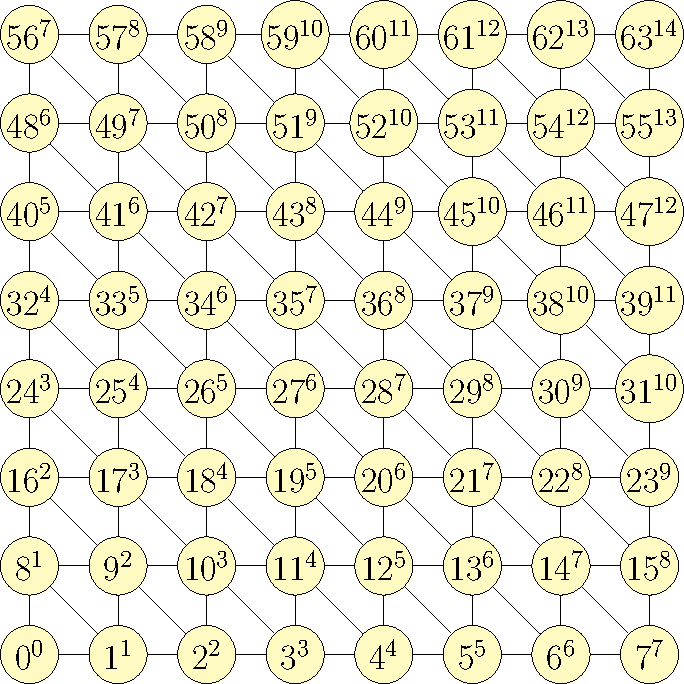
\includegraphics[height=0.18\textheight,width=0.32\textwidth]{pics/level_construction/stencil_2d_7pt}
			\begin{picture}(0,0)
			\put(-44,68){\fbox{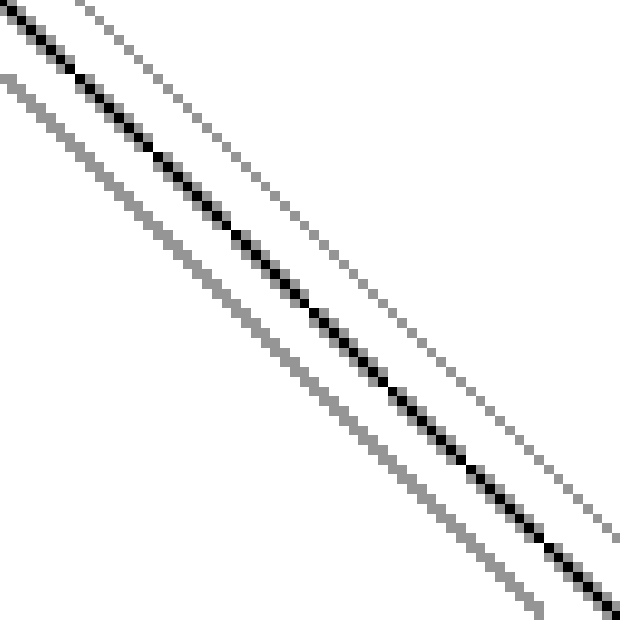
\includegraphics[height=1.4cm]{pics/level_construction/FDM_2d_7pt_non_perm}}}
			\end{picture}
		}
	\hspace{1em}
	\subfloat[Permuted graph ($G'$)]{\label{fig:2d_7pt_perm}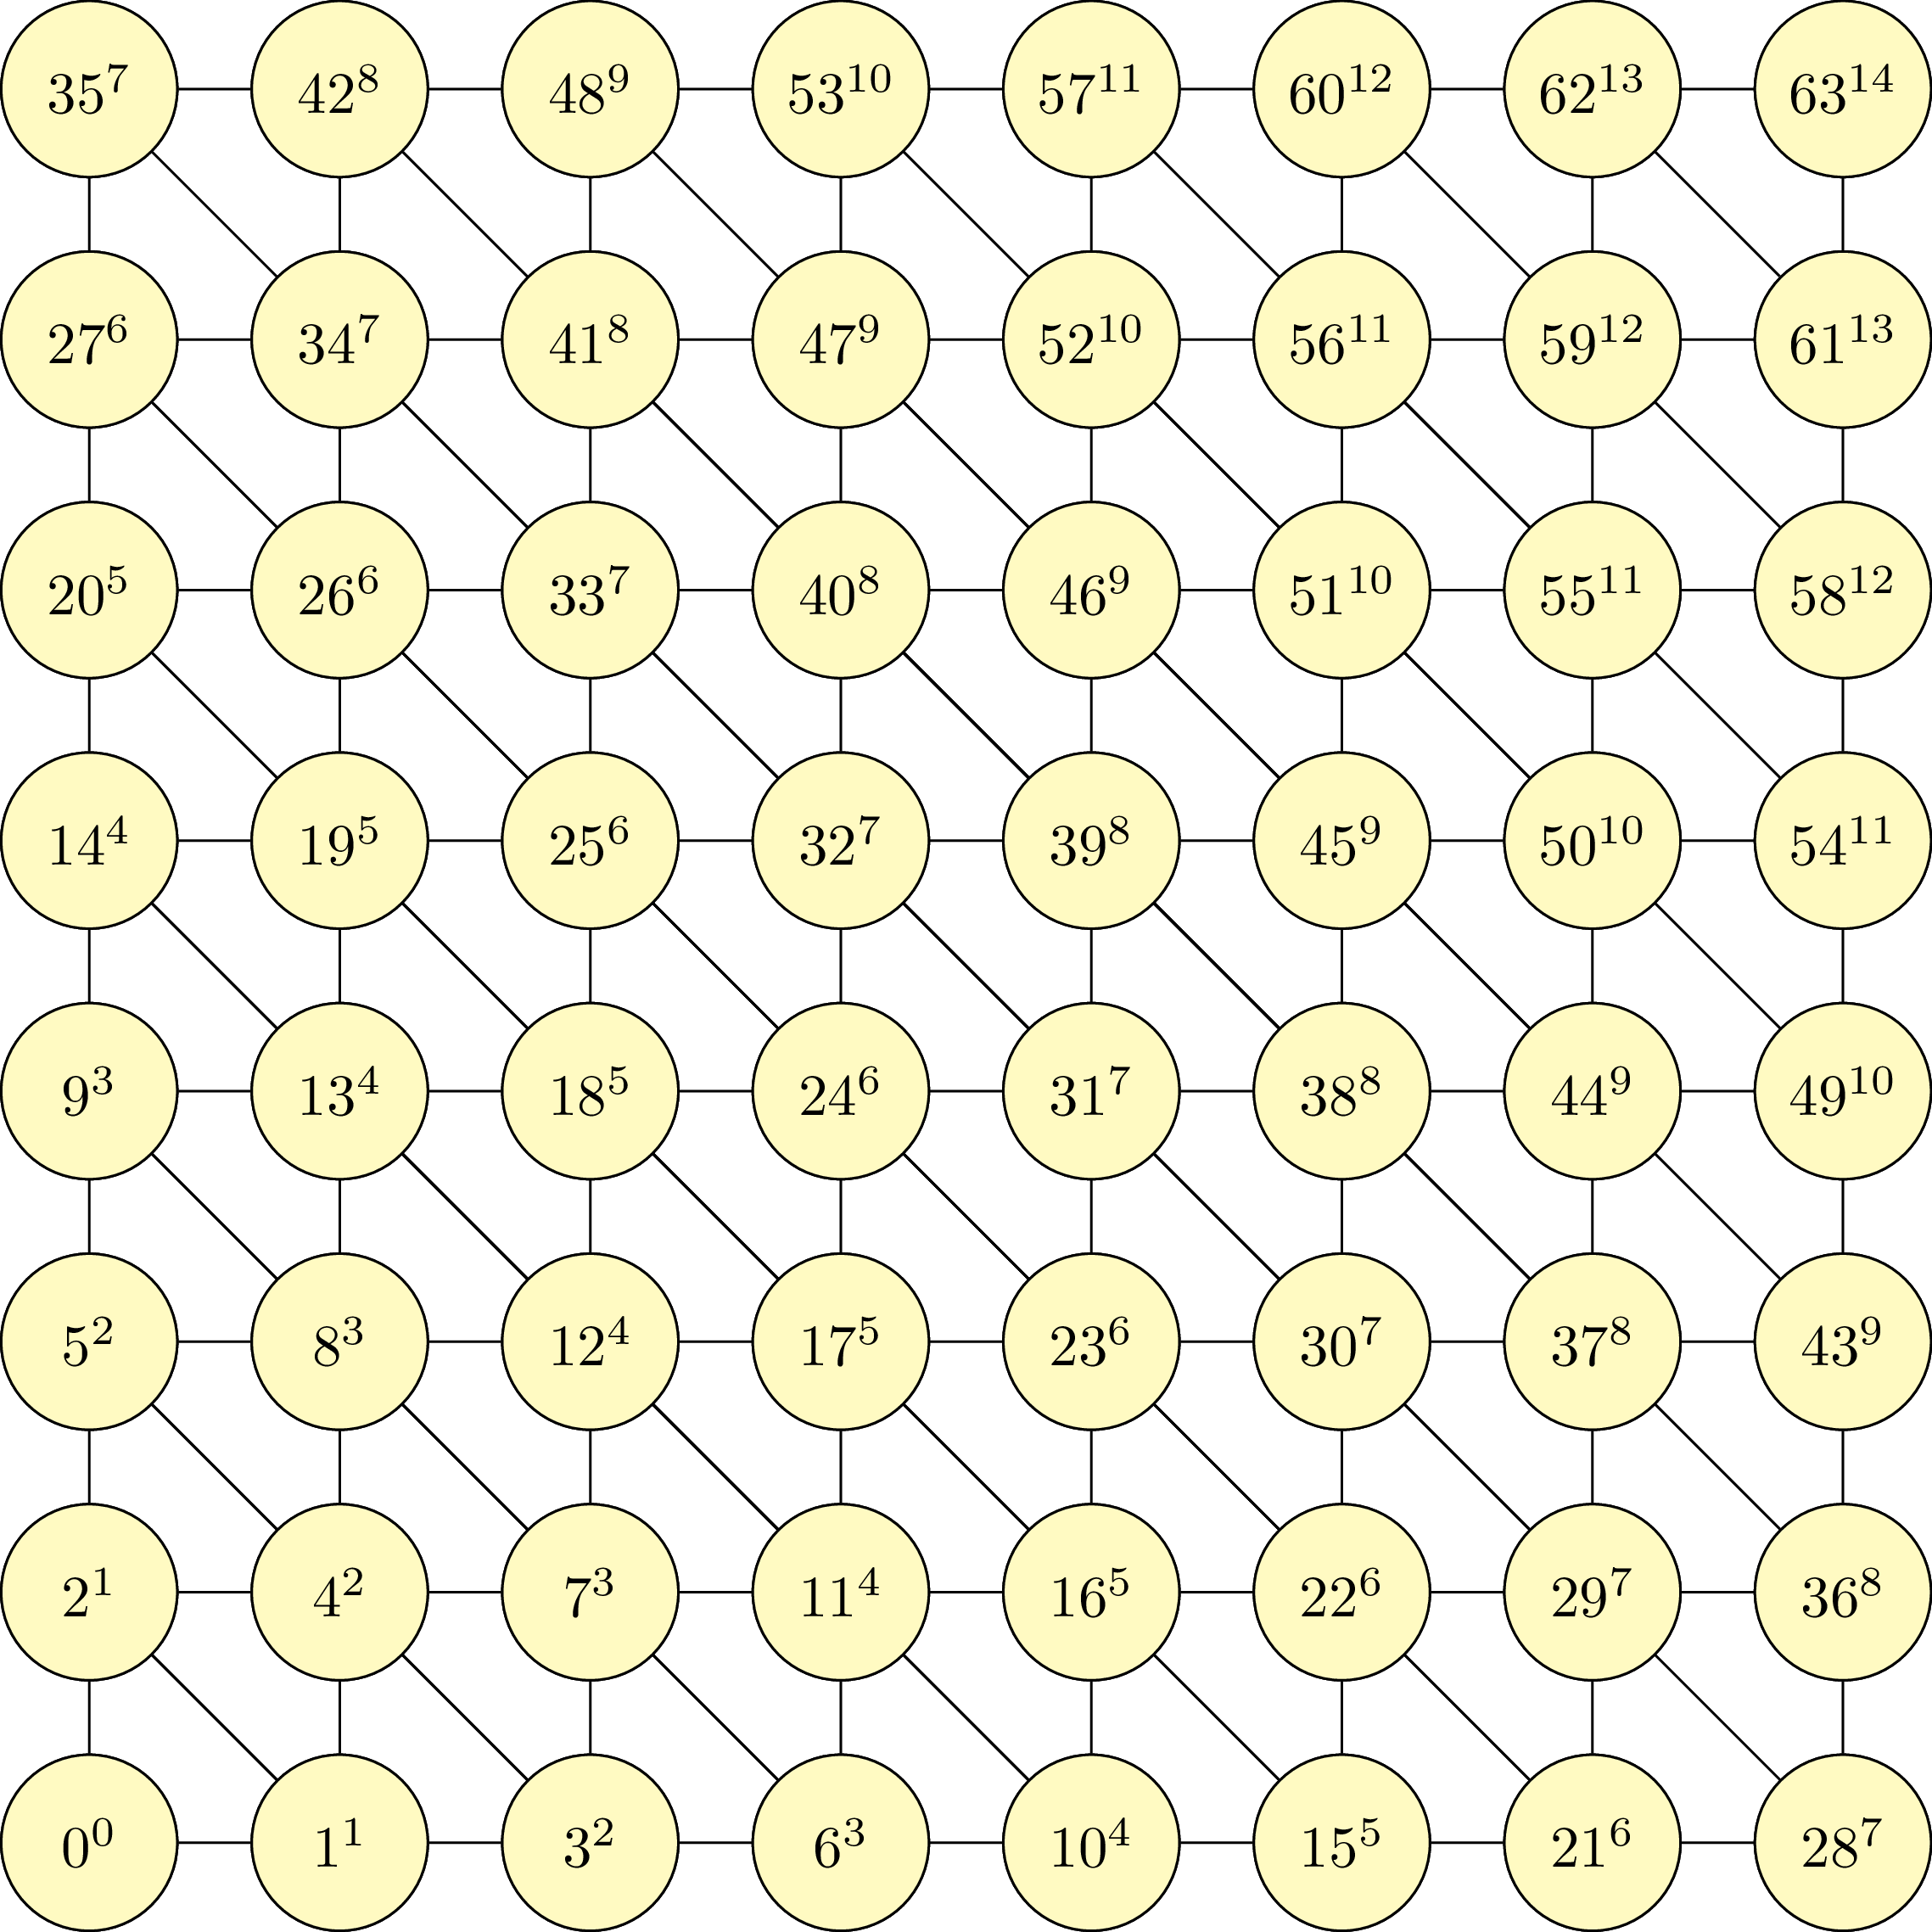
\includegraphics[height=0.18\textheight,width=0.32\textwidth]{pics/permutation/stencil_2d_7pt}
			\begin{picture}(0,0)
			\put(-43.5,68){\fbox{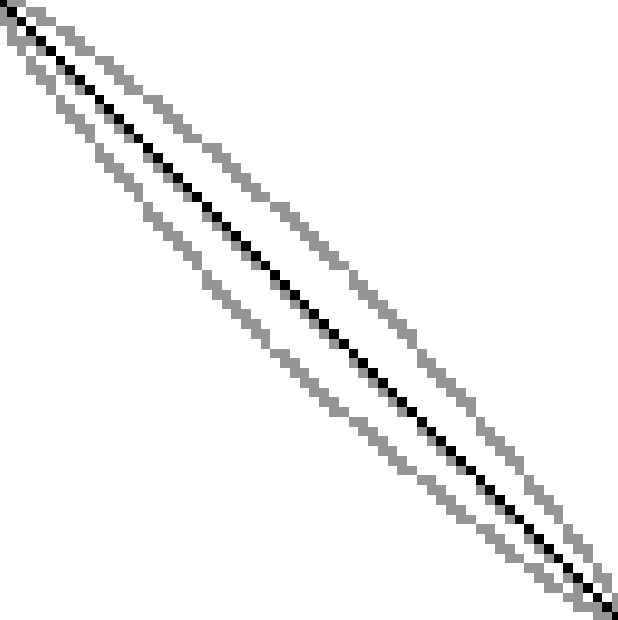
\includegraphics[height=1.4cm]{pics/permutation/FDM_2d_7pt_perm}}}
			\end{picture}
		}
	\hspace{1em}
	\subfloat[]{\label{fig:2d_7pt_levelPtr}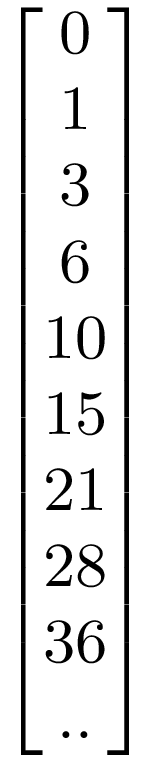
\includegraphics[height=0.18\textheight,width=0.07\textwidth]{pics/permutation/levelPtr}}
	\caption{\sref{fig:2d_7pt_level_construction} Levels of the original graph and \sref{fig:2d_7pt_perm} the permuted
          graph for the \stex. Insets show the corresponding sparsity patterns.
          \sref{fig:2d_7pt_levelPtr} Shows the entries of the \levelPtr array associated
          with $G'$.}
	\label{fig:2d-7pt_step_1_2}
\end{figure}


%\subsection{Permutation}\label{subsec:PERM}

After the \levels have been determined, the matrix is permuted in the
order of its \levels, such that the vertices in $L(i)$ are stored
consecutively and appear before those of
$L(i+1)$. \Cref{fig:2d-7pt_step_1_2} shows the graph ($G' = P(G)$)
of the \stex after applying this permutation ($P$) and demonstrates
the enhanced spatial locality of the vertices within and between
\levels (see \Cref{fig:2d_7pt_perm}) as compared to the original
(lexicographic) numbering (see \Cref{fig:2d_7pt_level_construction}).
Until now the procedure is the same as \acrshort{BFS} (or
\acrshort{RCM}).

As \acrshort{RACE} uses information about the \levels for resolving
dependencies in the coloring step, we store the index of the entry point to each
\level in the permuted data structure (of $G'$) in an array
$\levelPtr[0:$ \acrshort{totalLvl}$]$, so that \levels on $G'$ can be
identified as
\begin{equation*}
  L(i) = \set{ u : u \in [\levelPtr[i]:(\levelPtr[i+1]-1)]
    \text{ and } u \in V(G')}\eos
\end{equation*}
The entries of \levelPtr for the \stex are shown in \Cref{fig:2d_7pt_levelPtr}. 
%, and one could easily read from \levelPtr that vertices from $\levelPtr(4)=7$ to $\levelPtr(5)-1=10$ belongs to $L(4)$.
 
\subsection{Distance-k coloring} \label{subsec:DK}

The data structure generated above serves as the basis for our \DK coloring
procedure as it contains information about the neighborhood relation
between the vertices of any two \levels. Following the definition
in~\cite{dist_k_def}, two vertices are called \DK neighbors if the
shortest path connecting them consists of at most $k$ edges.
%In this section we introduce the idea of \DK neighbor and show how
%this idea can be used to color the matrix with the help of the level
%information that we already have in hand.
This implies that $u$ is a \DK neighbor of $v$ (referred to as
$u\xrightarrow{k}v$) if
\begin{equation}\label{eq:dk}
  u\xrightarrow{k}v  \iff  v \in \set{ u \cup N(u) \cup N^2(u) \cup \cdots N^k(u) }\eos
\end{equation}
For the undirected graphs as used here, $u\xrightarrow{k}v$
also implies $v\xrightarrow{k}u$. Based on this definition we consider
two vertices to be \DK independent if they are not \DK
neighbors, and two \levels are said to be \DK independent 
%if the vertices between them are \DK independent. 
if their vertices are mutually \DK independent.
Thus, \levels $L(i)$ and $L(i\pm(k+j))$ of the permuted
graph $G'$ are \DK independent for all $j\geq1$, denoted as
\begin{equation}\label{corollary_dk}
	L(i) \not{\xrightarrow{k}} L(i\pm(k+j)) \forall j\geq1 \eos
\end{equation} 

\begin{comment}
 as shown in the
following.
\begin{corollary}\label{corollary_dk}
$L(i)$ and $L(i\pm(k+j))$ are \DK independent $\forall j\geq1$. 
\end{corollary}
\begin{proof}
  We prove by contradiction. Let there exist $u,v \in V(G')$ such that
  $u \in L(i)$ and $v \in \bigcup\limits_{j\geq 1}L(i \pm (k+j))$. Assume $u,v$
  are \DK neighbors ($u\xrightarrow{k}v$). From \Cref{eq:level},
  \Cref{eq:dk}, and the fact $G'$ is undirected we get
\begin{align*}
  u\xrightarrow{k}v \iff & v \in \set{L(i) \cup L(i \pm 1) \cup \cdots \cup L(i \pm k)} \\
  \implies & v \notin L(i \pm (k+j)) \text{  } \forall j \geq 1\cma
\end{align*}
which contradicts our assumption about $v$\@.
Thus it follows that $u$ and $v$ are \DK independent.
\end{proof}
\end{comment}

\Cref{corollary_dk} implies that if there is a gap of at least
one \level between any two \levels (e.g., $L(i) \mbox{ and } L(i+2)$) all
pairs of vertices between these two levels are \DONE independent. Similarly
if the gap consists of at least two \levels between any two
\levels (e.g., $L(i) \mbox{ and } L(i+3)$) we have \DTWO independent
\levels, and so on.
 \begin{figure}[t]
 	\centering
 	\subfloat[Distance-1 independent \levelGroups]{\label{fig:2d_7pt_d1}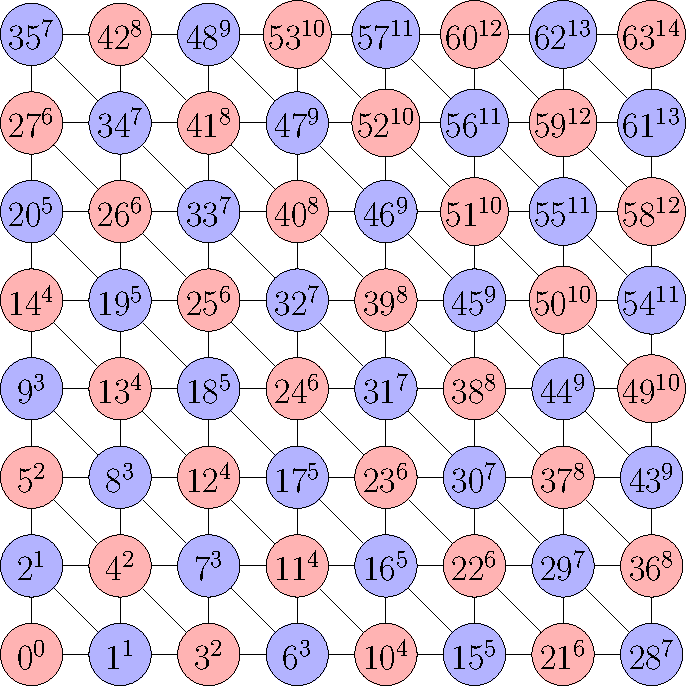
\includegraphics[height=0.2\textheight,width=0.4\textwidth]{pics/dk_coloring/stencil_2d_7pt_d1}}
 	\hspace{2.5em}
 	\subfloat[Distance-2 independent \levelGroups]{\label{fig:2d_7pt_d2}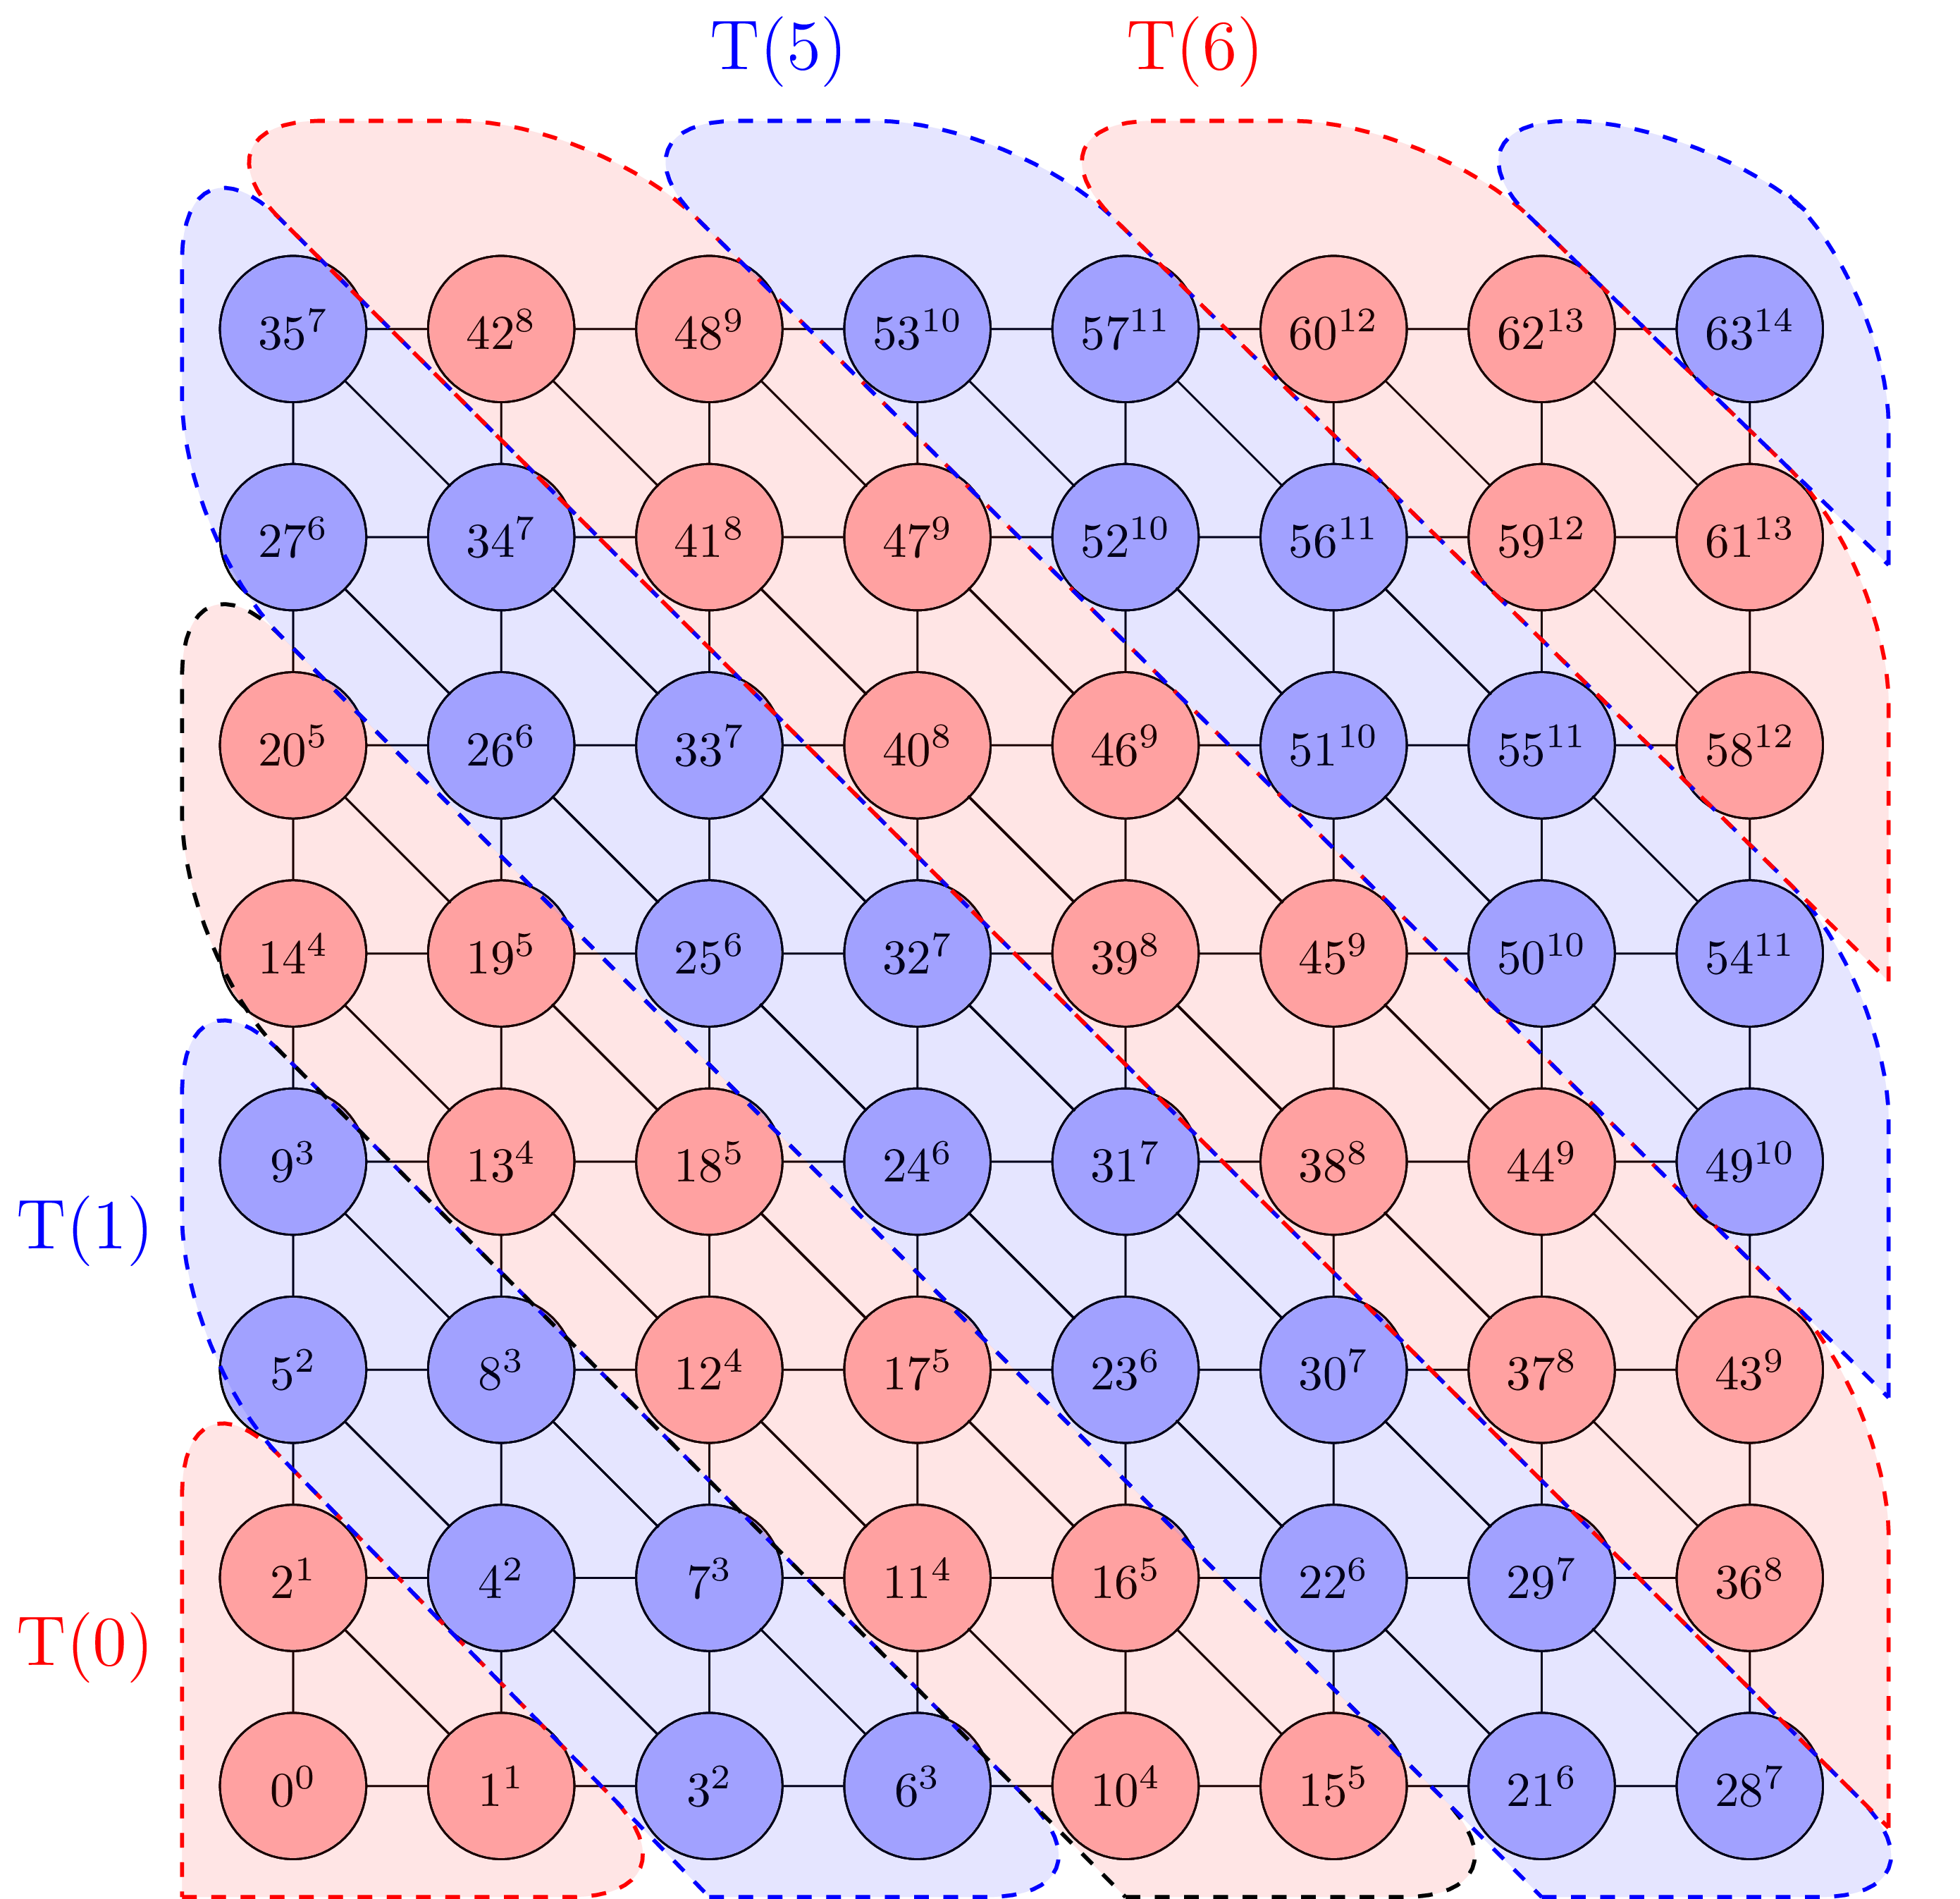
\includegraphics[height=0.23\textheight,width=0.48\textwidth]{pics/dk_coloring/stencil_2d_7pt_d2_with_lg}}
 	\caption{Forming \DONE and \DTWO independent \levelGroups for the \stex.}
 	\label{fig:2d-7pt_d1_d2}
 \end{figure}
 
 
The definition used in \Cref{corollary_dk} offers many choices for
forming \DK independent sets of vertices, which can then be executed
in parallel.  In \Cref{fig:2d-7pt_d1_d2} we present one example each
for \DONE (\Cref{fig:2d_7pt_d1}) and \DTWO (\Cref{fig:2d_7pt_d2})
colorings of our \stex. The \DONE coloring uses a straightforward
approach by assigning two colors to alternating \levels, i.e., \levels
of a color can be calculated concurrently. In case of \DTWO
independence we do not use three colors but rather aggregate two
adjacent \levels to form a \textit{\levelGroup} (denoted by
\acrshort{T_i}) and perform a \DONE coloring on top of those
groups. This guarantees that vertices of two \levelGroups of the same
color are \DTWO independent and can be executed in parallel. Here, the
vertices in $T(0)$, $T(2)$, $T(4)$, and $T(6)$ can be operated on by
four threads in parallel, i.e., one thread per \levelGroup.  After
synchronization the remaining four blue \levelGroups can also be
executed in parallel. This idea can be generalized such that for \DK
coloring, each \levelGroup contains $k$ adjacent \levels.
%\atleast $k$ adjacent \levels but
%the number of \levels  per \levelGroup may be different. 
Thus formed \levelGroups are then \DONE
colored. Then, all \levelGroups within a color can be executed in
parallel. This simple approach allows one to generate workload for
a maximum of ${\acrshort{totalLvl}}/{2 k}$ threads if \DK coloring is
requested.\footnote{\CAcomm{This implies as the number of levels increase 
so does the parallelism. For \eg if the matrix contains at least one dense row 
 it will have no parallelism, as $\acrshort{totalLvl}=2$ in this case.}} 
Note that in all cases vertices within a single \levelGroup
 are computed in their original order, which allows for good
spatial access locality.
 
Choosing the same number of \levels for each \levelGroup may
however cause severe load imbalance depending on the matrix structure. In
particular the use of bandwidth reduction schemes such as BFS or RCM
will further worsen that problem due to the lenslike shape of the
reordered matrix (see inset of \Cref{fig:2d_7pt_perm}), leading to low
workload for \levelGroups containing the top and bottom rows of the
  matrix. Compare, \eg $T(0)$ and $T(7)$ with $T(3)$ and $T(4)$ in
\Cref{fig:2d_7pt_d2}. However, \Cref{corollary_dk} does not require
exactly $k$ levels to be in a \levelGroup but  
requires only ``\atleast'' k \levels in a \levelGroup. In
the following we exploit this to alleviate the imbalance
problem.
 %coloring by aggregating consecutive levels into \levelGroups (denoted by $T(i)$). In  \Cref{fig:2d_7pt_d1}  and \Cref{fig:2d_7pt_d2} we present one example for \DONE and \DTWO coloring of our \stex, respectively. The \DONE coloring uses straight forward approach by assigning two colors to alternating levels, i.e. \levelGroup and \level is equivalent here. For and applying a \DONE coloring on top of those groups as shown for \DTWO coloring in \Cref{fig:2d_7pt_d2}.  In this context \Cref{fig:2d-7pt_d1_d2} contains two potential colorings for \DONE independent \levels as \DTWO coloring also solves \DONE dependencies.  One could also group some more of nearby \levels together to form a \levelGroup, and make this \DONE or \DTWO independent of other \levelGroups. The $i$-th \levelGroup would be denoted by $T(i)$. Difference between \level and  \levelGroup can be seen in \Cref{fig:2d_7pt_d2}, for \Cref{fig:2d_7pt_d1} \levelGroup and \level coincides. In principle one could compute on all independent \levelGroups in parallel, but sequentially within a \levelGroup, \ie for example in \Cref{fig:2d_7pt_d2} $T(0)$, $T(2)$, $T(4)$, $T(6)$ can be operated by four different threads in parallel and in the next sweep rest \levelGroups. For the configurations seen in \Cref{fig:2d-7pt_d1_d2} then we have $\frac{\acrshort{totalLvl}}{2}$ and $\frac{\acrshort{totalLvl}}{4}$ parallelism for \DONE and \DTWO kernels respectively.
 %However the problem with the configurations like the one seen in \Cref{fig:2d-7pt_d1_d2} {\CA is that there, check Holger's comment} is load imbalances between threads because the number of rows (\nrows) per \levelGroup is not distributed evenly. As seen here in the case of \stex the threads working on extreme ends of graph (\eg $T(1), T(7)$) have a small amount of work compared to the threads working on middle (\eg $T(3), T(4)$). 
  
  \subsection{Load balancing}\label{subsec:LB} 
The RACE load balancing scheme tries to balance the workload between level groups 
within each color for a given number of threads while maintaining data locality 
and \DK constraint between the two colors. To achieve this we use an idea
similar to incremental graph partitioning \cite{load_balancing}. 
The \levelGroups containing low workload grab adjacent levels from neighboring
 level groups and overloaded level groups shift levels to adjacent level groups. 
 As a target for the load balancing scheme one can balance the number of rows (\ie vertices) 
 of the \levelGroups ($\acrshort{nrows}(T(i))$)  or the number of nonzeros (\ie edges) of the 
 \levelGroups ($\acrshort{nnz}(T(i))$). Both variants are supported by our implementation 
 and we choose balancing by the number of rows in the following to demonstrate our load 
 balancing algorithm, which can be found in \Cref{alg:LB}.
%Depending on the matrix each \levelGroup contains different number of rows, that leads to load imbalances as seen above in \Cref{subsec:DK}. \Inorder to avoid this problem we employ a load balancing scheme. At this step  we plug in details from the hardware side  namely the total parallelism required by the hardware. The idea is to exploit only the required parallelism while at the same time maintain \DK constraint seen in \Cref{corollary_dk}. To balance the load more nearby \levels would be added to a \levelGroup ($T(x)$) which has less number of rows ($\nrowsMath(T(x))$) and at \levelGroup where we have considerably big \levels only sufficient amount of \levels to maintain \DK constraint would be assigned. Assigning nearby levels instead of others further helps in preserving data locality. 
 
Our algorithm tries to reduce the variances of the workload in the level groups, \ie the number of rows ($\acrshort{nrows}(T(i))$) in each \levelGroup $T(i)$. For a given set of \levelGroups we calculate the mean and variance of $\acrshort{nrows}(T(i))$ within each color, \ie red and blue colors.  
 %For example in \Cref{fig:2d_7pt_d2} we need to calculate mean of $T\_size$ of all \levelGroups in red sweep and blue sweep separately. 
The overall variance, which is the target of our minimization procedure, is then found by summing up the variances between colors. \Inorder to reduce this value we first select the two \levelGroups with largest negative/positive deviation from the mean {(which is $T(5)$ and $T(4)$ in step 1 of \Cref{fig:lb_alg}) and try to add/remove levels to/from these \levelGroups (see top row of \Cref{fig:lb_alg}). When removing \levels from a \levelGroup one has to take care that the \DK coloring is not violated by keeping at least $k$ levels in a \levelGroup. The shift of \levels is done via a pointer array denoted as $T\_ptr$, which points to the beginning of each \levelGroup (see \Cref{fig:lb_alg}), avoiding any copy operation. If shifting levels between the two level groups with the largest deviation does not lead to a lower overall variance, no levels are exchanged and we choose the next pair of level groups according to a ranking which is based on the absolute deviation from the mean (see \Cref{alg:LB} for implementation details) and continue. Doing this process in an iterative way we finally end up in a state with the lowest overall variance at which no further moves are possible either due to a violation of \DK dependency or an increase in overall variance. \Cref{fig:lb_alg} shows the load balancing procedure under a \DTWO constraint for some initial mapping of 17 levels to six level groups. Applying the procedure to our  \stex of size $16 \times 16$  requesting \DTWO coloring and ten level groups leads to the mapping shown in \Cref{fig:2d_7pt_lb}. Note that \levelGroups at the extreme ends have more \levels due to fewer vertices (\acrshort{nrows}) in each \level, while \levelGroups in the middle having more vertices maintain two levels to preserve the \DTWO constraint.
%One could also do this entire load balancing based on number of nonzeros (\acrshort{nnz}) rather than \nrows, in this case $T\_size(i)=\acrshort{nnz}(T(i))$ (nonzeros in $T(i)$).
  
   \begin{figure}[t]
   	\centering
   	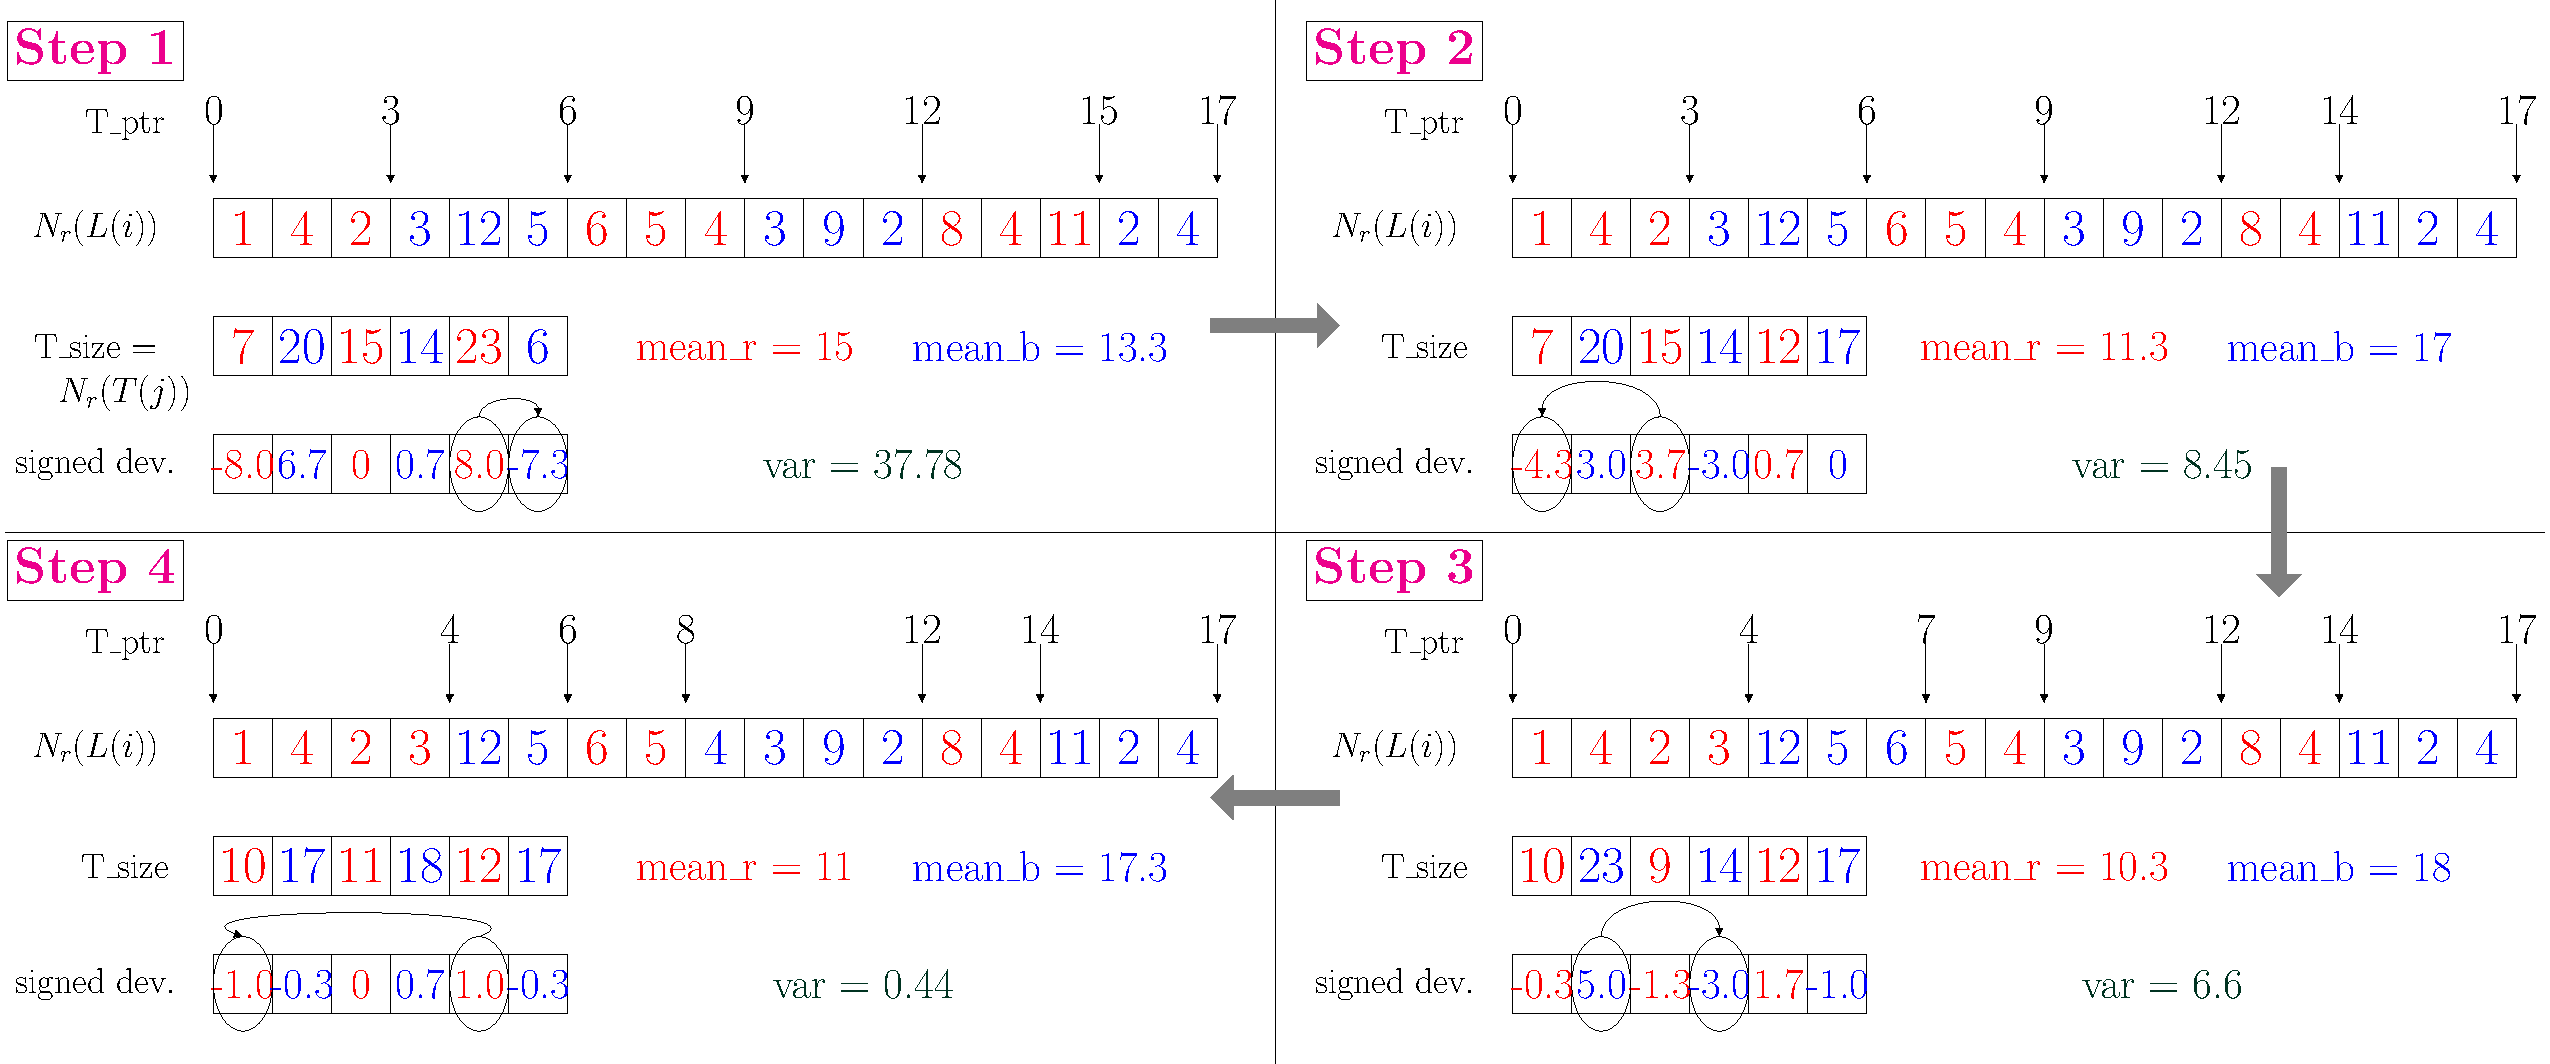
\includegraphics[height=0.22\textheight,width=\textwidth]{pics/load_balancing/lb_alg/lb_all}
   	\caption{All steps of the load balancing scheme applied to an arbitrarily chosen initial distribution of 17 levels into six level groups for \DTWO coloring. Rebalancing steps are performed clockwise starting from top-left. $mean\_r$ and $mean\_b$ denote the current average number of rows per \levelGroup and color. $var$ is the overall  variance}
   	\label{fig:lb_alg}
   \end{figure}
   
   \begin{figure}[t]
	   	\centering
	   	\subfloat[Five threads]{\label{fig:2d_7pt_lb}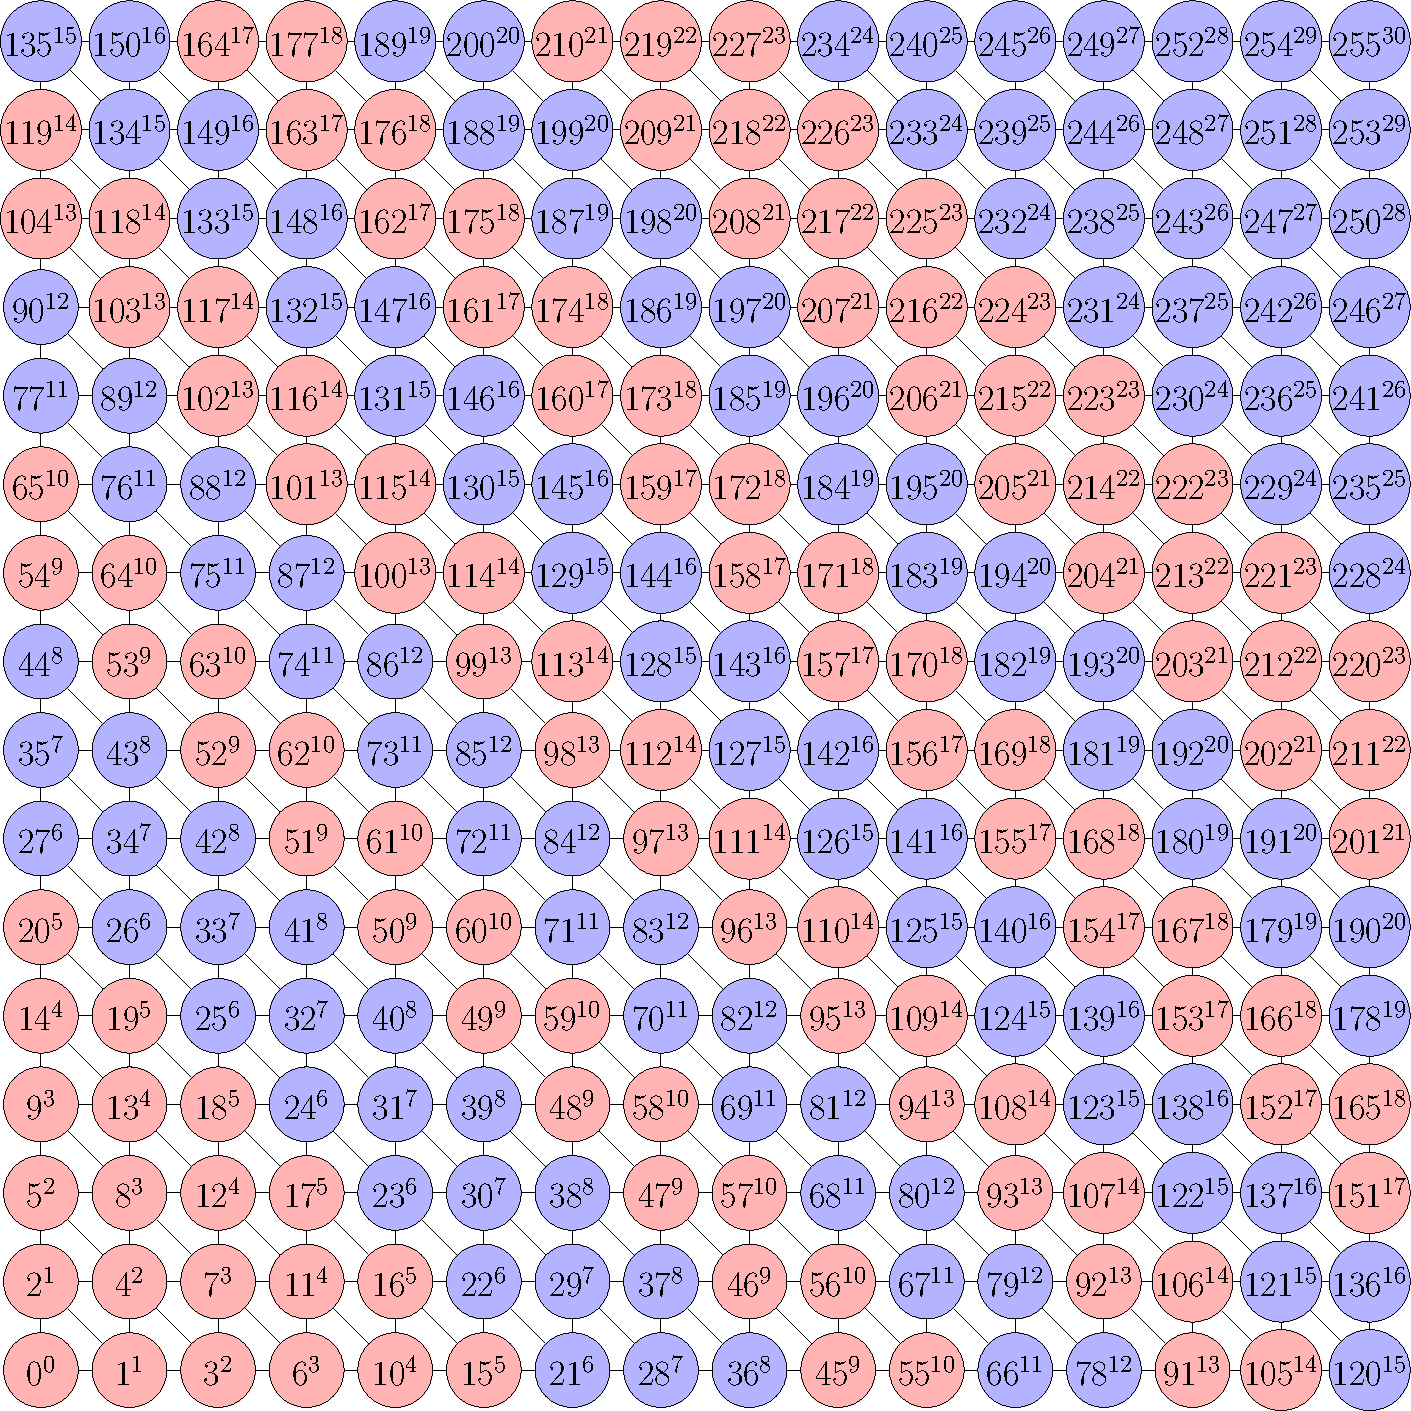
\includegraphics[width=0.48\textwidth, height=0.28\textheight]{pics/load_balancing/2d-7pt/stencil_2d_7pt}}
	   	\hspace{0.2em}
	   	\subfloat[Eight threads]{\label{fig:2d_7pt_lb_8_threads}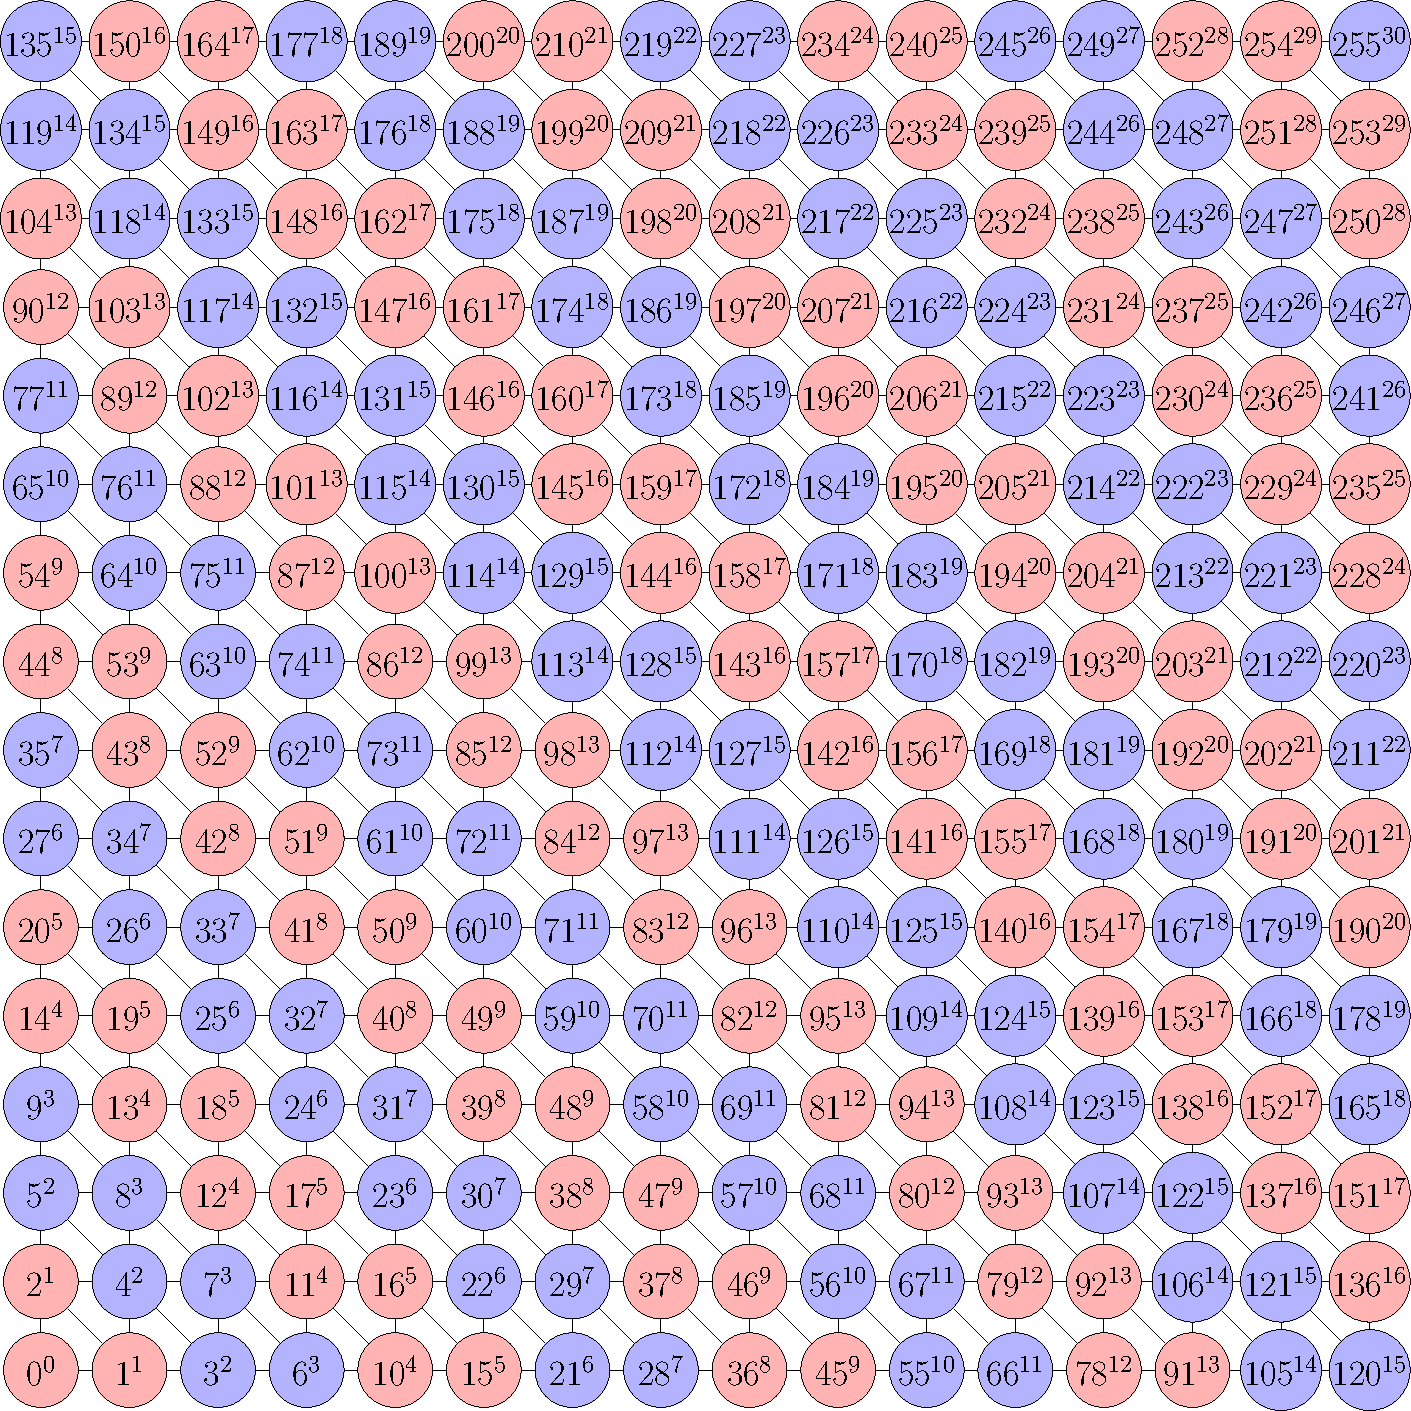
\includegraphics[width=0.48\textwidth, height=0.28\textheight]{pics/load_balancing/2d-7pt/stencil_2d_7pt_8_threads}}
		 \caption{\sref{fig:2d_7pt_lb} after load balancing for five threads and \DTWO dependency for the \stex, domain size $16 \times 16$. 
		 	%Note that \levelGroups at extreme end have more \levels due to fewer \acrshort{nrows} in each \level, while \levelGroups in the middle having bigger \levels maintain two levels to preserve \DTWO constraint. 
		 \sref{fig:2d_7pt_lb_8_threads} after load balancing for eight threads.
		}
	\end{figure}
   

%    \begin{figure}
%      \begin{minipage}[c]{0.63\textwidth}
%      	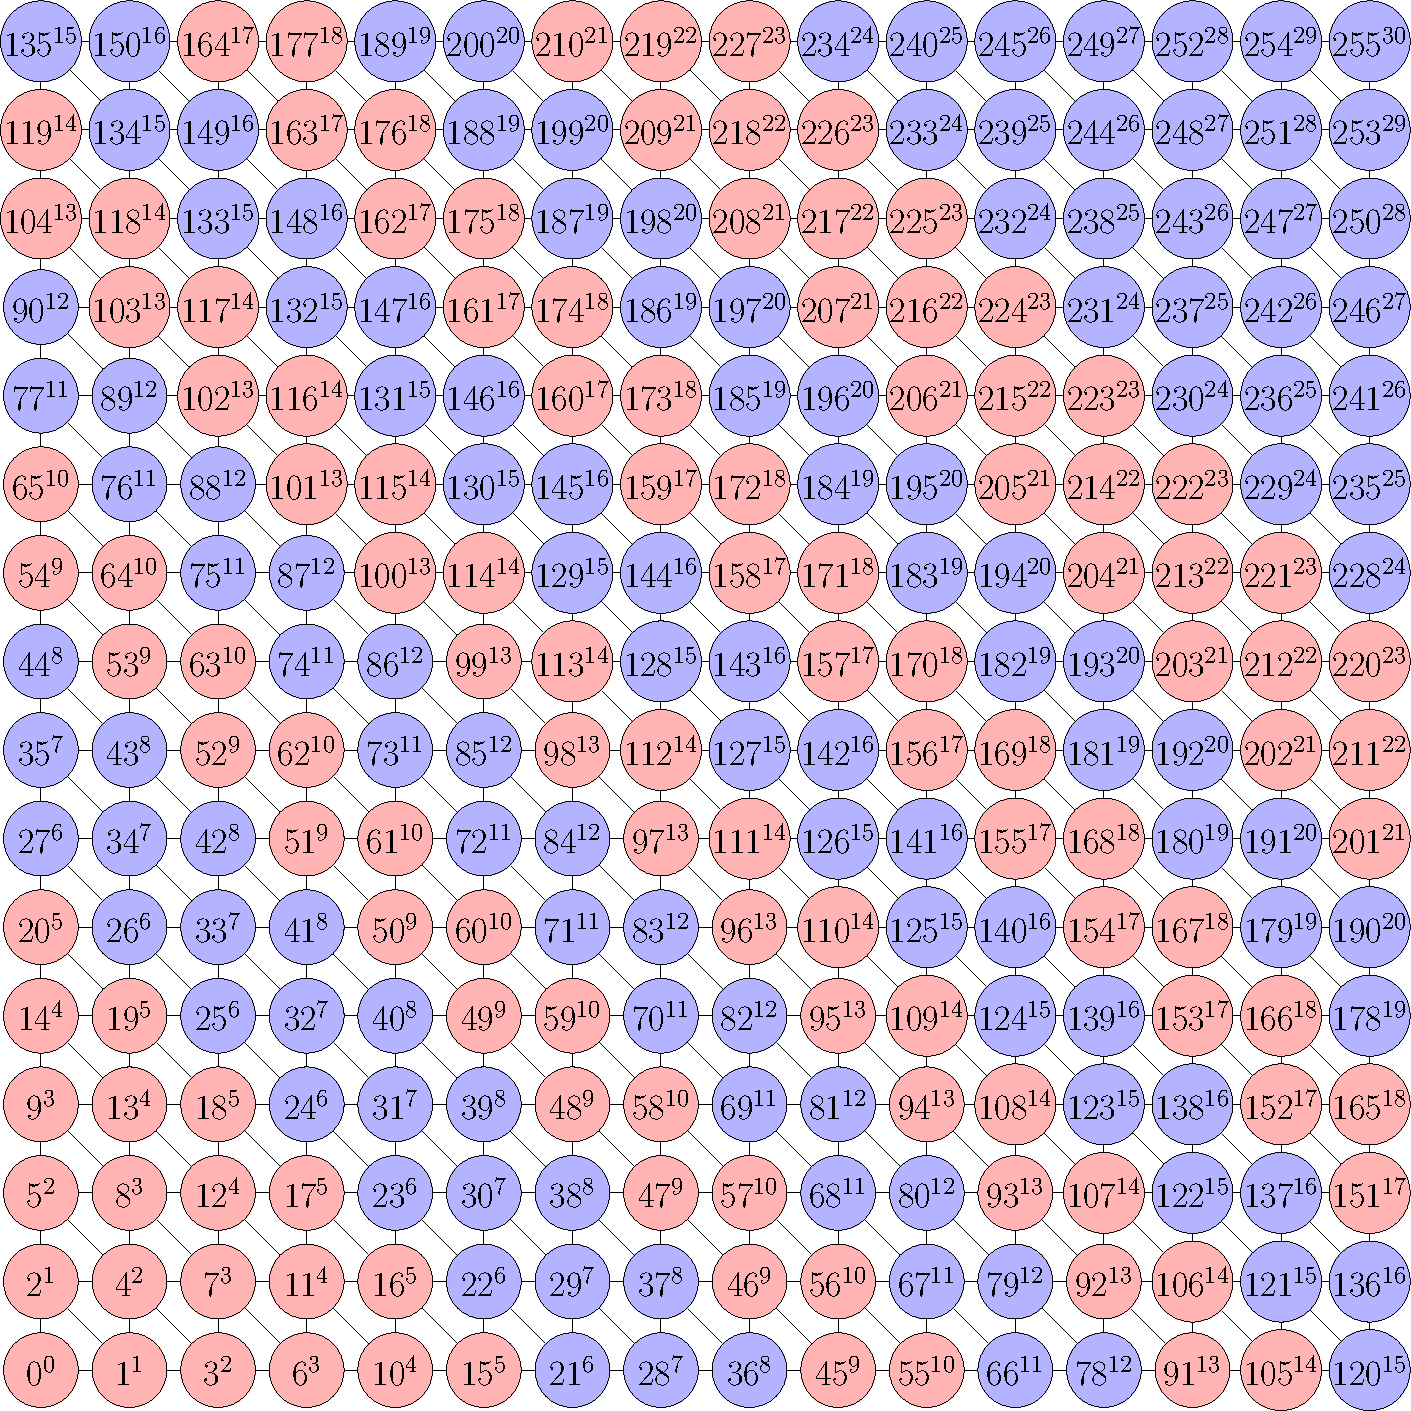
\includegraphics[height=0.26\textheight,width=0.9\textwidth]{pics/load_balancing/2d-7pt/stencil_2d_7pt}
%      \end{minipage}\hfill
%      \begin{minipage}[c]{0.34\textwidth}
%      	\caption{After load balancing for five threads and \DTWO dependency on \stex, domain size $16 \times 16$. Note that \levelGroups at extreme end have more \levels due to fewer \acrshort{nrows} in each \level, while \levelGroups in the middle having bigger \levels maintain two levels to preserve \DTWO constraint.
%      	} \label{fig:2d_7pt_lb}
%      \end{minipage}
%     \end{figure}
%  
%      \begin{figure}
%      	\begin{minipage}[c]{0.63\textwidth}
%      		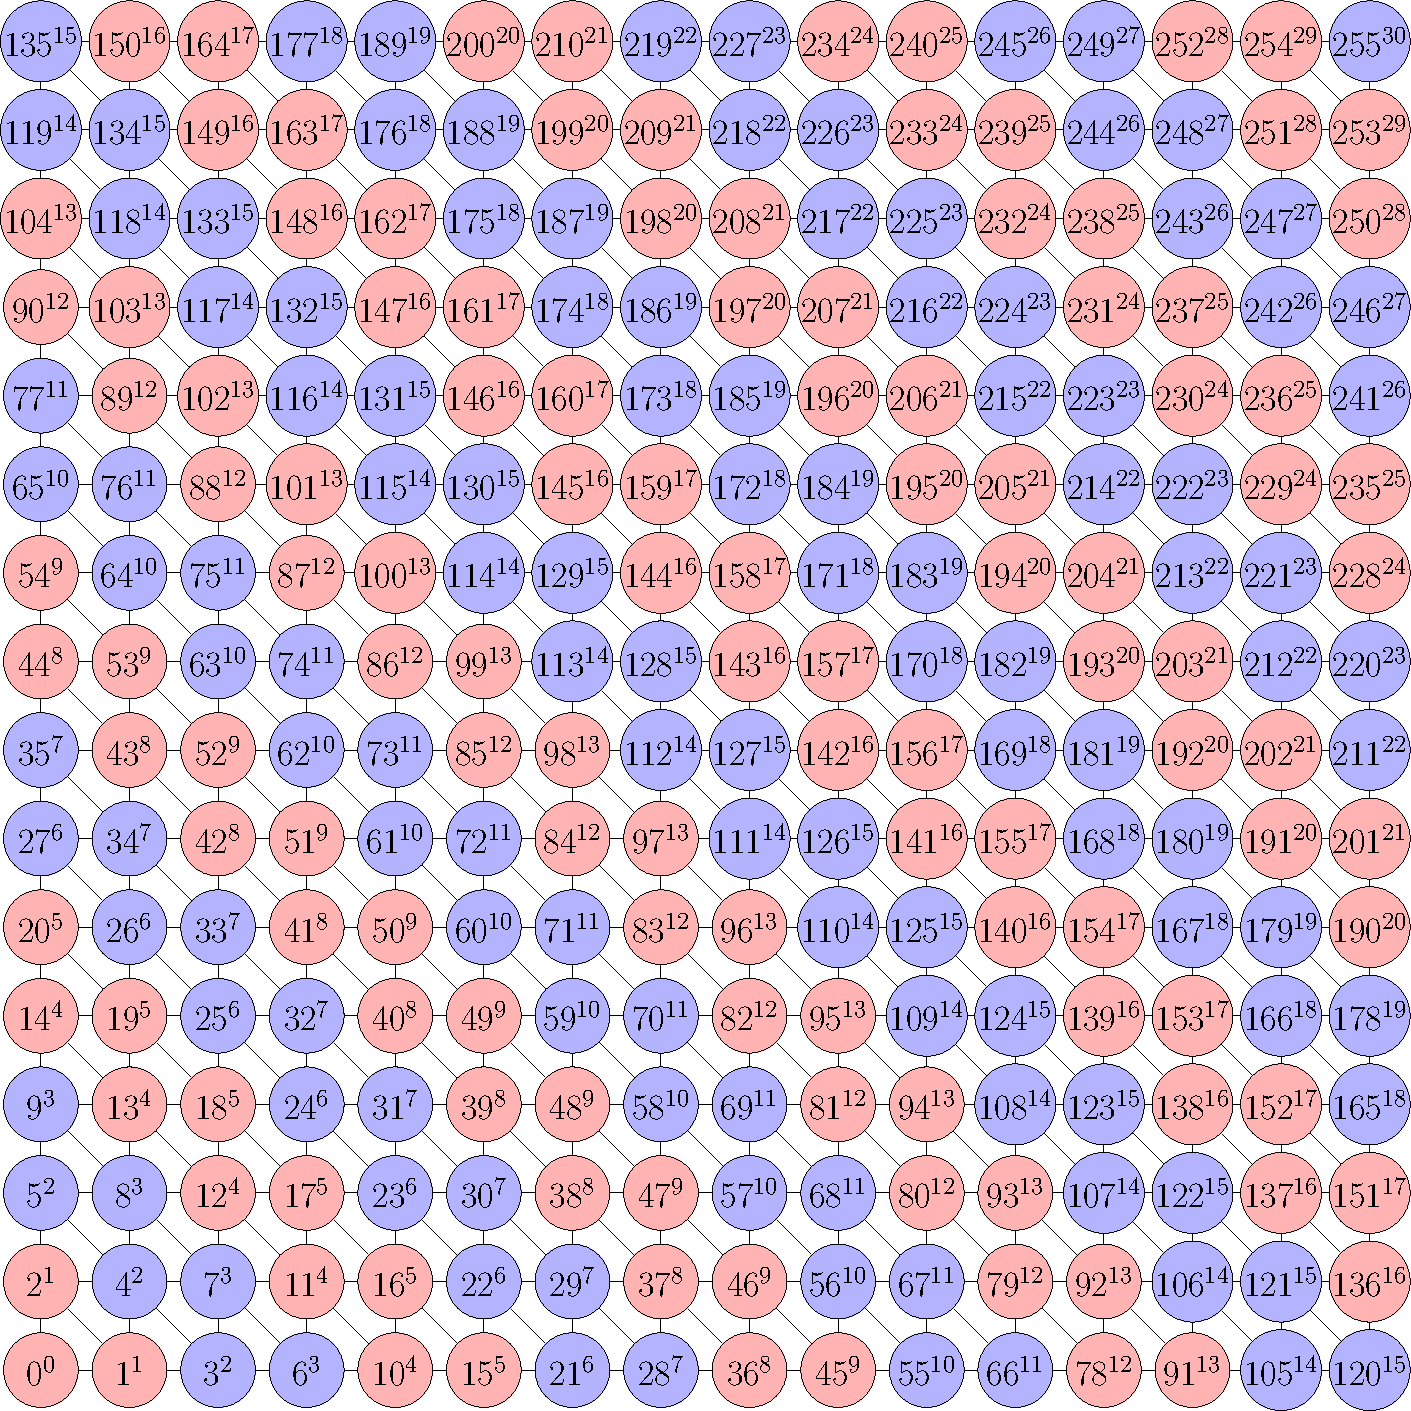
\includegraphics[height=0.26\textheight,width=0.9\textwidth]{pics/load_balancing/2d-7pt/stencil_2d_7pt_8_threads}
%      	\end{minipage}\hfill
%      	\begin{minipage}[c]{0.34\textwidth}
%      		\caption{After load balancing for eight threads and \DTWO dependency on \stex, domain size $16 \times 16$. Note the massive load imbalance between the \levelGroups at extreme ends and in 
%      			the middle. \CAcomm{I am not sure whether we need this, it consumes lot of space and we could explain it with a sentence. TODO: Explain it somewhere}}
%      		 \label{fig:2d_7pt_lb_8_threads}
%      	\end{minipage}
%      \end{figure}  


	\subsection{Recursion}\label{subsec:REC}
As discussed in \Cref{subsec:DK} the maximum degree of parallelism is limited
by the total number of levels (\acrshort{totalLvl}) and may be further reduced 
by level aggregation in the load balancing step. In case of
	stencil $16\times16$ example the maximum possible parallelism 
	is eight threads which may lead to load imbalance as seen in 
	\Cref{fig:2d_7pt_lb_8_threads}.
	%For example
	%requesting the maximum possible eight threads instead of five 
	%threads (\Cref{fig:2d_7pt_lb}) for the stencil $16\times16$ example, 
	%it results in massive load imbalance as seen in \Cref{fig:2d_7pt_lb_8_threads}. 
Therefore, %to match the high levels of parallelism in modern compute devices 
we need to search for 
further parallelism within the \levelGroups.  Compared to methods like \acrshort{MC} 
we didn't require all vertices in a \levelGroup to be \DONE (or \DK in general) 
independent of each other, which is a consequence of our \level based approach 
where we required \DK independency between vertices of different levels but not 
within a level (see \Cref{corollary_dk}). There can exist more parallelism within 
the \levelGroups which we can interpret as \subgraphs.  Thus, we apply the three 
steps of our method recursively on selected \subgraphs to exploit the parallelism 
within them.  
%i.e.  \levelGroups which are recursively refined will be computed by multiple threads whereas unmodified \levelGroups will be assigned to a single thread. 

In the following we first demonstrate in \Cref{subsec:D1_dependency} the basic idea in the context of \DONE dependencies where all dependencies can be resolved within the given \levelGroup by design. However, for $k>1$, vertices in a \levelGroup may have \DK dependencies through vertices in adjacent \levelGroups. We generalize our procedure to \DK dependencies as a second step in \Cref{subsec:Dk_dependency}. Finally, in \Cref{subsec:subgraph_selection} we apply the recursive scheme to our \stex and introduce proper \subgraph selection as well as global load balancing strategies. 

In order to visualize the basic concepts easily and discuss important corner cases of the recursive approach we start with the simple graph shown in \Cref{fig:rec_d1_s1_a}, which is not correlated to our \stex. To distinguish between \levelGroups at different stages \acrshort{s} of our recursive procedure we add a subscript to the levels (\acrshort{L_si}) and \levelGroups (\acrshort{T_si}) indicating the stage of recursion at which they are generated, with $s=0$ being the original distribution before recursion is applied to any \subgraph. 

%also for most of the graphs as we approach the limit of parallelism there is not much room for load balancing, leading to imbalances. Depending on matrix and hardware underneath this might lead to inefficient utilization of resources. \Inorder to avoid this problem we use the concept of recursion and exploit further parallelism if required by the hardware. Idea here is to intelligently select sub-graph(s) of the entire matrix and apply all the three steps recursively on this \subgraph. In the following we will show this concept in the context of \DONE and  later we will extent it to \DK dependencies. In order to explain the basic concepts easily and include all the corner cases we demonstrate the procedure on a simple graph which is shown in \Cref{fig:rec_d1_s1_a}, later we will show the results of applying recursion on \stex. Further we will discuss on the method employed to select proper sub-graph and to have a globally balanced load.
	
	\subsubsection{Distance-$1$ dependency} \label{subsec:D1_dependency}
%\LevelGroups which we constructed till now belong to first stage of recursion ($s=0$). Stage number of recursion is denoted using subscript, \ie for example $L_s(i)$ denotes \level $i$ of stage $s$. Contrary to methods like \acrfull{MC} we didn't require each nodes in a color to be \DONE independent of each other, rather we had a weak constraint as prescribed by \Cref{corollary_dk}. Due to this there can exist more parallelism within a \levelGroup. 

For the \DONE coloring of the graph in \Cref{fig:rec_d1_s1} we find that the third \levelGroup of the initial stage (T$_0$(2)) still contains vertices which are \DONE independent, \eg vertices $3 \not{\xrightarrow{1}} 4$ ($3$  \DONE independent to $4$), $3 \not{\xrightarrow{1}} 5$, $3 \not{\xrightarrow{1}} 6$, and $4 \not{\xrightarrow{1}} 6$, implying each of these pairs can be computed in parallel without any \DONE conflicts. This parallelism has not been exploited in the first stage ($s=0$)  as vertices in $L_0(i)$ (here $i=2$) are chosen such that they are \DONE neighbors of \level $L_0(i-1)$ ignoring any vertex relations in $L_0(i)$. 
%We now apply our method recursively to the levels or \levelGroups to identify further paralleism within them.  	
     \begin{figure}[t]
     	\centering
     	\subfloat[Example graph]{\label{fig:rec_d1_s1_a}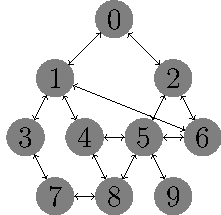
\includegraphics[width=0.26\textwidth, height=0.14\textheight]{pics/recursion/d1/rec_graph_s1/recursion_graph_1}}
     	\hspace{1.5em}
     	\subfloat[Stage 0, levels in graph]{\label{fig:rec_d1_s1_b}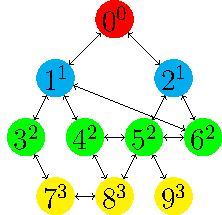
\includegraphics[width=0.26\textwidth, height=0.14\textheight]{pics/recursion/d1/rec_graph_s1/recursion_graph_2}}
     	\hspace{1.5em}
     	\subfloat[\DONE coloring]{\label{fig:rec_d1_s1_c}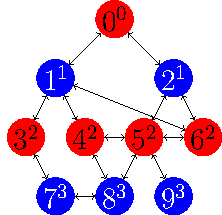
\includegraphics[width=0.26\textwidth, height=0.14\textheight]{pics/recursion/d1/rec_graph_s1/recursion_graph_3}}
        \caption{Shows potential for more parallelism. $T_0(1),T_0(2),$ and $T_0(3)$ have more parallelism. Note that the graph shown here is not related to the previous \stex.}
     	\label{fig:rec_d1_s1}
     \end{figure}

Recursion starts with the selection of a \subgraph of the matrix, which is discussed in more detail later (see \Cref{subsec:subgraph_selection}). Here we choose a \subgraph induced by $T_0(2)$. The  \subgraph can be isolated from the rest of the graph since the \DONE coloring step in stage 0 has already made \levelGroups independent of each other. Now we just need to repeat the three steps explained previously (\Cref{subsec:LEVEL_CONST}--\Cref{subsec:LB}) on this \subgraph.
%to exploit parallelism within this \subgraph.
   
     \begin{figure}[t]
     	\centering
     	\subfloat[]{\label{fig:rec_d1_s2_a}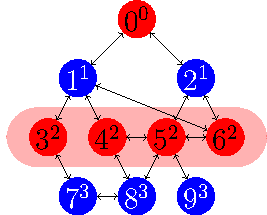
\includegraphics[width=0.28\textwidth, height=0.14\textheight]{pics/recursion/d1/rec_graph_s2/recursion_graph_stage2_1}}
     	\hspace{2.25em}
     	\subfloat[]{\label{fig:rec_d1_s2_b}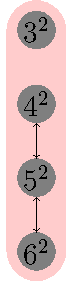
\includegraphics[width=0.07\textwidth, height=0.14\textheight]{pics/recursion/d1/rec_graph_s2/recursion_graph_stage2_2}}
     	\hspace{1.75em}
     	\subfloat[]{\label{fig:rec_d1_s2_c}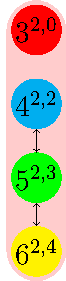
\includegraphics[width=0.065\textwidth, height=0.14\textheight]{pics/recursion/d1/rec_graph_s2/recursion_graph_stage2_3}}
     	\hspace{1.75em}
     	\subfloat[]{\label{fig:rec_d1_s2_d}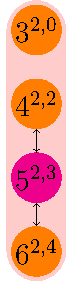
\includegraphics[width=0.065\textwidth, height=0.14\textheight]{pics/recursion/d1/rec_graph_s2/recursion_graph_stage2_4}}
	     \hspace{1.75em}
	     \subfloat[]{\label{fig:rec_d1_s2_e}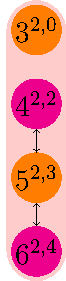
\includegraphics[width=0.065\textwidth, height=0.14\textheight]{pics/recursion/d1/rec_graph_s2/recursion_graph_stage2_5}}
     	\caption{Applying recursion to the \subgraph induced by $T_0(2)$. \Cref{fig:rec_d1_s2_b} shows the isolated \subgraph, \Cref{fig:rec_d1_s2_c} presents the level construction step on the \subgraph. Two potential \DONE colorings of this  \subgraph are shown in \Cref{fig:rec_d1_s2_d,fig:rec_d1_s2_e}.}
     	
     	\label{fig:rec_d1_s2}
     \end{figure}
     
     \Cref{fig:rec_d1_s2} shows an illustration of applying the first recursive step ($s=1$) on $T_0(2)$, where we extend the definition of the vertex numbering in \Cref{eq:node_notation} to the following:
	 \begin{equation}
	    v^{i,j,k...} \implies v \in \set{L_0(i) \cap L_1(j) \cap L_2(k) \cap \cdots}.
	 \end{equation}
	 
     In this case at the end of the recursion (\cf \Cref{fig:rec_d1_s2_d,fig:rec_d1_s2_e}) on $T_0(2)$ we obtain parallelism for two more threads. Note that the \subgraphs might have islands (group of vertices that are not connected to the rest of the graph), \eg vertex 3 and vertices 4,5,6 form two islands in \Cref{fig:rec_d1_s2_b}. Since an island is totally disconnected from the rest of the (sub)graph it can be executed in parallel to the rest of the (sub)graph. To take advantage of this the starting node in the next island is assigned with an increment of two levels, as seen in \Cref{fig:rec_d1_s2_c}. Therefore multiple valid \DONE configurations (\cf \Cref{fig:rec_d1_s2_d,fig:rec_d1_s2_e}) exist and the selection of the optimal one will be done in the final load balancing step as described in \Cref{subsec:LB}.    
     
     With this recursive process we were able to find independent \levelGroups ($T_{s+1}$) within a \levelGroup of the previous stage ($T_s$) and therefore the thread which works on $T_s$ has to spawn threads to parallelize within $T_{s+1}$.
     
	\subsubsection{Distance-$k$ dependencies with $k>1$}  \label{subsec:Dk_dependency}
In general, however, it is not sufficient in the recursion step to consider only the \subgraphs induced by \levelGroups as can be seen in \Cref{fig:rec_d2_wrong_a} for \DTWO coloring. Applying  the three steps (see \Cref{fig:rec_d2_wrong_b,fig:rec_d2_wrong_c,fig:rec_d2_wrong_d})  to  the \subgraph induced by $T_0(1)$ does not guarantee \DTWO independence between the new \levelGroups $T_1(0)$ and $T_1(2)$. It is obvious that for general \DK colorings two vertices $a,b$ within a \levelGroup might be connected by a shared vertex $c$ outside the \levelGroup.  Thus, our three step procedure must be applied to a \subgraph which contains the actual \levelGroup ($T_s(j)$) as well as its all distance-$p$ neighbors, where $p=1,2,\ldots,(k-1)$.
%as they
%For \DK the same procedure as \DONE applies, except with a slight difference in selecting the \subgraph. In \DONE we considered \subgraphs induced by \levelGroups, but for \DK coloring this is not sufficient. As seen in \Cref{fig:rec_d2_wrong_a} for \DTWO coloring the selection of $T_0(1)$ as \subgraph and applying the three steps (see \Cref{fig:rec_d2_wrong_b}, \Cref{fig:rec_d2_wrong_c} and \Cref{fig:rec_d2_wrong_d}) did not guarantee \DTWO independency within \levelGroup $T_1$ of the \subgraph, for \eg $T_1(0)$ and $T_1(2)$ are not \DTWO independent (\cf \Cref{fig:rec_d2_wrong_d}). This is due to the fact that for $k>1$ dependencies two vertices $a,b$ within a \subgraph might be connected to a common vertex ($c$) outside the \subgraph leading to a \DK dependency between $a$ and $b$. In \Cref{fig:rec_d2_wrong} we see 	$3 \xrightarrow{1} 1 \text{ \& } 6 \xrightarrow{1} 1 	\implies 3 \xrightarrow{2} 6$, but since vertex $1$ was not in the \subgraph considered we missed this dependency. 
     \begin{figure}[t]
     	\centering
     	\subfloat[]{\label{fig:rec_d2_wrong_a}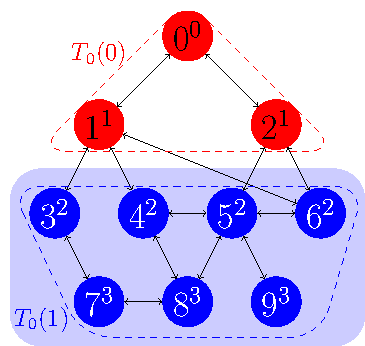
\includegraphics[width=0.23\textwidth, height=0.13\textheight]{pics/recursion/d2/wrong/recursion_graph_wrong_1}}
     	\hspace{0.6em}
     	\subfloat[]{\label{fig:rec_d2_wrong_b}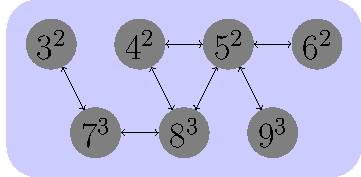
\includegraphics[width=0.23\textwidth, height=0.07\textheight]{pics/recursion/d2/wrong/recursion_graph_wrong_2}}
     	\hspace{0.6em}
     	\subfloat[]{\label{fig:rec_d2_wrong_c}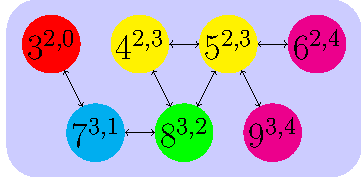
\includegraphics[width=0.23\textwidth, height=0.07\textheight]{pics/recursion/d2/wrong/recursion_graph_wrong_3}}
     	\hspace{0.6em}
     	\subfloat[]{\label{fig:rec_d2_wrong_d}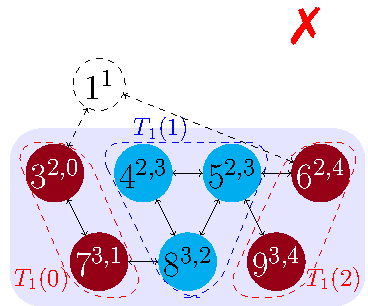
\includegraphics[width=0.23\textwidth, height=0.13\textheight]{pics/recursion/d2/wrong/recursion_graph_wrong_4}}
     	\caption{Two \levelGroups generated by a \DTWO coloring (\Cref{fig:rec_d2_wrong_a}). \Cref{fig:rec_d2_wrong_b} shows the \subgraph induced by \levelGroup $T_0(1)$. Level construction on the selected \subgraph is shown in \Cref{fig:rec_d2_wrong_c}. Forming \DTWO independent \levelGroups on these levels does not guarantee a \DTWO independence between the newly generated \levelGroups of the same sweep (color) as seen in \Cref{fig:rec_d2_wrong_d}.}
     	\label{fig:rec_d2_wrong}
     \end{figure}

%\begin{equation*}
%	   N^{k-1}(T_s(j)) = \set{u : u \xrightarrow{k-1} v \text{  } \forall v \in T_s(j) \text { and } u \notin T_s(j)}.
%\end{equation*}

This ensures that there is no vertex outside the \subgraph which can mediate a \DK dependency between vertices in the embedded \levelGroup ($T_s(j)$). We can now construct the new levels on this \subgraph considering the neighborhood but only store the vertices in the new \levels $L_{s+1}(:)$ which are in the embedded \levelGroup ($T_s(j)$). Next we apply \DK coloring by aggregation of the new levels leading to a set of \levelGroups $T_{s+1}(:)$ within $T_s(j)$. \Cref{fig:rec_d2_correct} uses this approach to resolve the conflict demonstrated in \Cref{fig:rec_d2_wrong_d}. \Cref{fig:rec_d2_correct_b} presents the \subgraph containing the selected \levelGroup $T_0(1)$ and its \DONE neighborhood. %For \DTWO this would mean we have to include $1^{st}$ interface level, the new selection is illustrated in \Cref{fig:rec_d2_correct} (note the region shaded in blue). If we then do all the three steps with the newly created \subgraph, the final result will preserve \DTWO coloring (see \Cref{fig:rec_d2_correct_c}). In the example it can be observed vertices $3$ and $6$ which previously had same color now get assigned to different colors (see \Cref{fig:rec_d2_correct_d}). Note that the interface levels have to be considered only in the first step namely level construction in the rest of the steps we just need to consider target \subgraphs induced by the \levelGroups \ie in \Cref{fig:rec_d2_correct} the \subgraph induced by $T_0(1)$.   
\begin{figure}[t]
     	\centering
     	\subfloat[]{\label{fig:rec_d2_correct_a}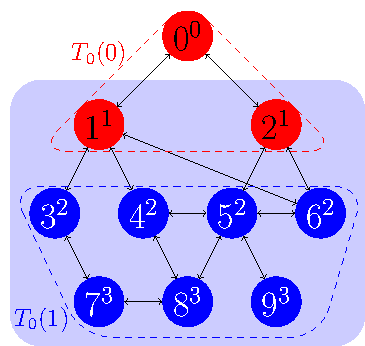
\includegraphics[width=0.22\textwidth, height=0.13\textheight]{pics/recursion/d2/correct/recursion_graph_correct_1}}
     	\hspace{0.6em}
     	\subfloat[]{\label{fig:rec_d2_correct_b}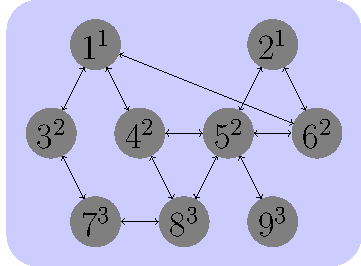
\includegraphics[width=0.22\textwidth, height=0.105\textheight]{pics/recursion/d2/correct/recursion_graph_correct_2}}
     	\hspace{0.6em}
     	\subfloat[]{\label{fig:rec_d2_correct_c}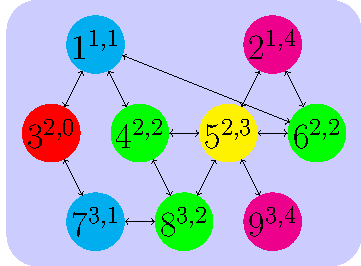
\includegraphics[width=0.22\textwidth, height=0.105\textheight]{pics/recursion/d2/correct/recursion_graph_correct_3}}
     	\hspace{0.6em}
     	\subfloat[]{\label{fig:rec_d2_correct_d}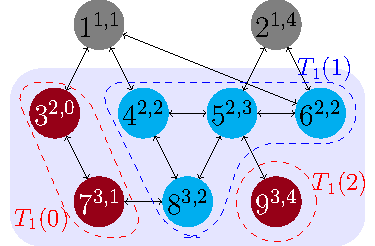
\includegraphics[width=0.22\textwidth, height=0.105\textheight]{pics/recursion/d2/correct/recursion_graph_correct_4}}
     	\hspace{0.6em}
     	\caption{Correct procedure for \DTWO coloring of \levelGroup $T_0(1)$. The \subgraph as shown in \Cref{fig:rec_d2_correct_b} contains \levelGroup $T_0(1)$ and its \DONE neighborhood. A level construction step is applied to this \subgraph in \Cref{fig:rec_d2_correct_c}. Distance-2 coloring by level aggregation leading to \levelGroups of stage 1 is shown in \Cref{fig:rec_d2_correct_d}; we get three \levelGroups at the end of the recursion on $T_0(1)$.}
     	\label{fig:rec_d2_correct}
     \end{figure}
Level construction is performed on the \subgraph (\Cref{fig:rec_d2_correct_c}) but the new levels only contain vertices of  $T_0(1)$, \ie $L_1(1) = \{7^{3,1}\}$. Finally, \DTWO coloring by aggregation of two adjacent levels is performed, leading to three \levelGroups of the second stage $s=1$ (\Cref{fig:rec_d2_correct_d}), \ie $T_1(0)=\{L_1(0) \cup L_1(1)\}$.  Now vertices $3$ and $6$ are mapped to \levelGroups of different colors. Note, that the permutation step on the newly generated levels is not shown but is performed as well to maintain data locality. 
    
%We finally apply the recursive step to the coloring shown in \Cref{fig:2d_7pt_lb} where parallelism is restricted to five threads at a time.  To increase parallelism to eight threads we do apply our recursive approach 
%Requesting parallelism for eight threads for our \stex with \DTWO independency instead of five threads (see result of our procedure applying one recursive step to \levelGroups $T_0(4),T_0(5),T_0(6)$ and $T_0(7)$ is seen in \Cref{fig:rec_2d-7pt_graph} (left). 
%In \Cref{fig:rec_2d-7pt_graph} we demonstrate the impact of one recursive step applied to our \stex with \DTWO 
       \begin{figure}[t]
       	\begin{minipage}[c]{0.6\textwidth}
       		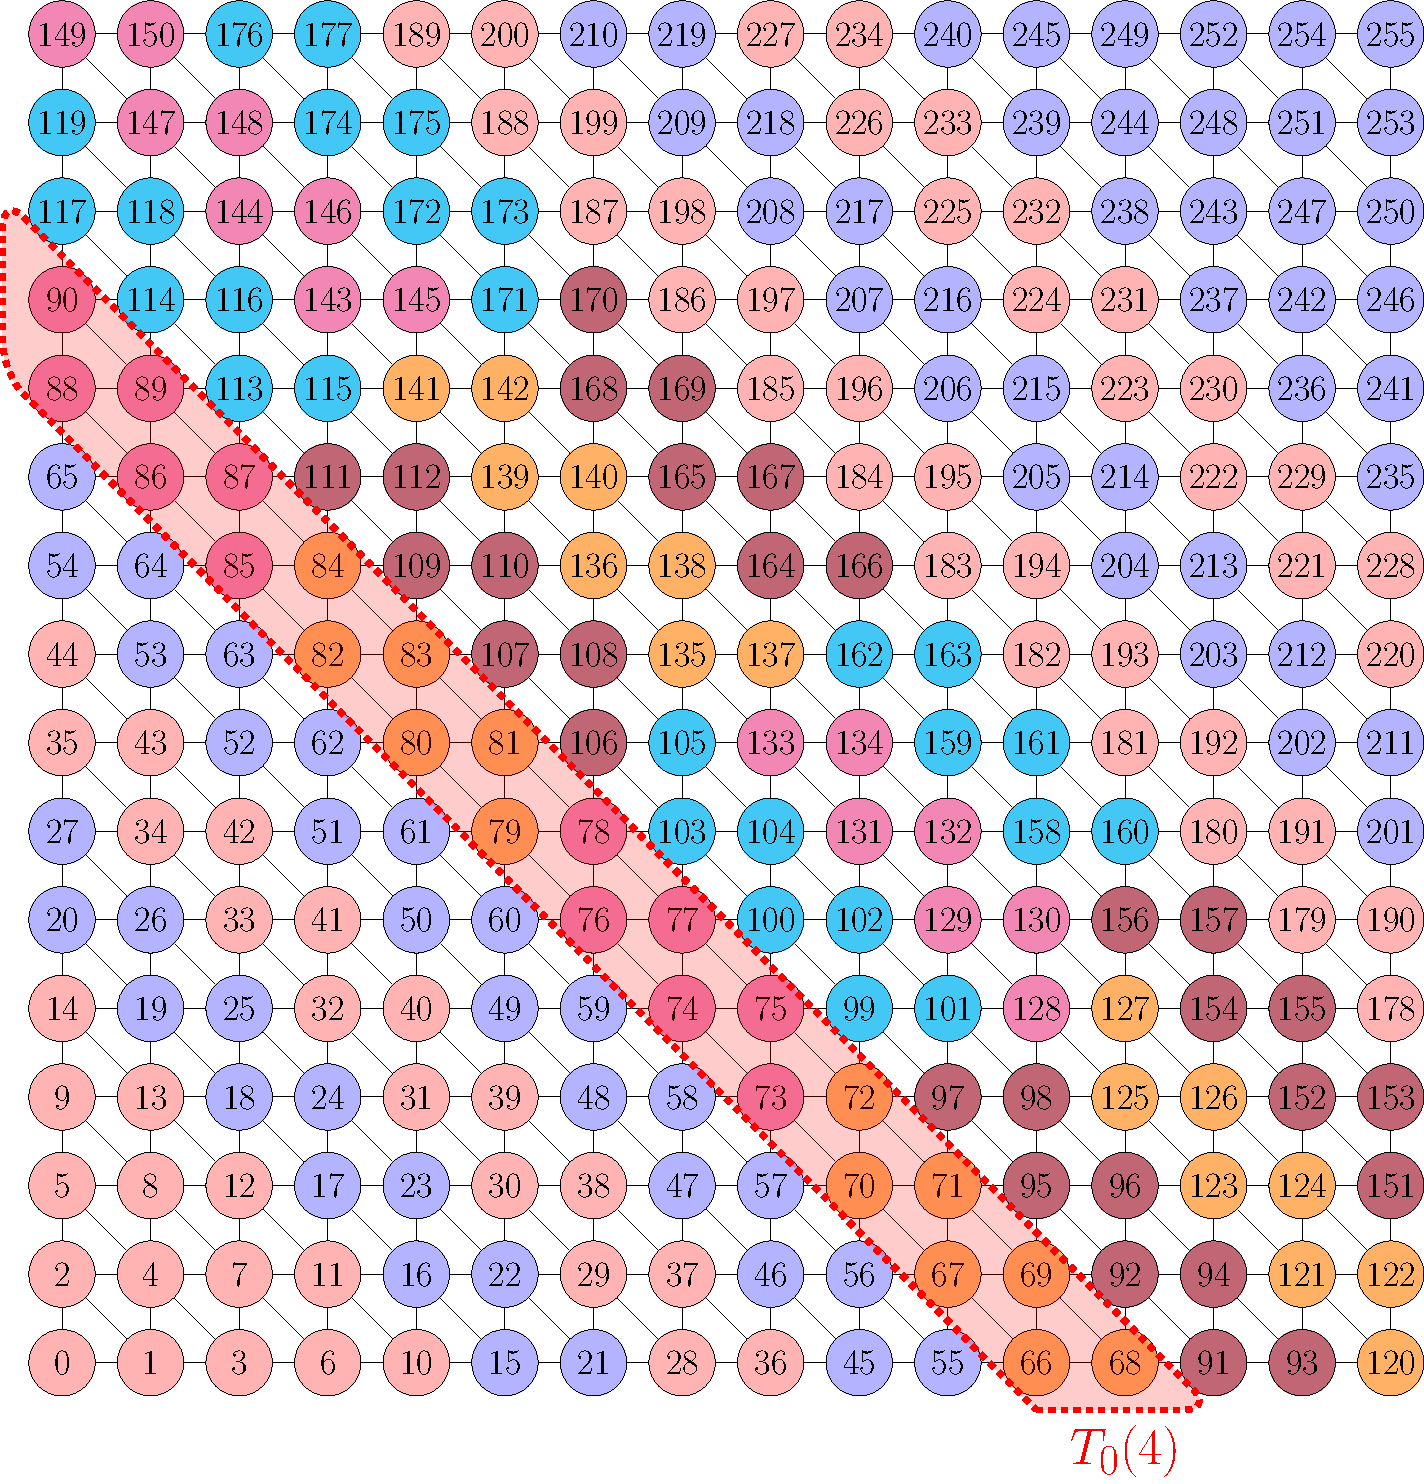
\includegraphics[height=0.3\textheight,width=0.89\textwidth]{pics/recursion/2d-7pt_example/2d-7pt/stencil_2d_7pt}
       	\end{minipage}\hfill
       	\begin{minipage}[c]{0.4\textwidth}
       	%	{\tt for parallel all \textcolor{red}{red}\\
       	%		\hspace*{1em} for parallel all \textcolor{amber}{orange}\\
       	%		\hspace*{1em} for parallel all \textcolor{magenta}{pink}\\
       	%	}
       	%	{\tt for parallel all \textcolor{blue}{blue}\\
       	%		\hspace*{1em} for parallel all \textcolor{carmine}{brown}\\
       	%		\hspace*{1em} for parallel all \textcolor{cyan}{cyan}\\
       	%	}
	       	\begin{tabular}{l|l}
	    %   		\toprule
	       		{Initial Stage} & {Recursion}\\
	       		{($s=0$)} & {($s=1$)}\\
	       		\midrule
	       	   \multirow{2}{*}{\textcolor{red}{red}} & {\textcolor{amber}{orange}}\\
	       	   \rule{0pt}{3ex}
	       	   %\cmidrule(lr){2-2}
	       		& {\textcolor{magenta}{pink}}\\
				\rule{0pt}{4ex} 
	       	   \multirow{2}{*}{\textcolor{blue}{blue}} & {\textcolor{carmine}{brown}}\\
	       	   %\cmidrule(lr){2-2}
	       	   \rule{0pt}{3ex}
	       	   & {\textcolor{cyan}{cyan}}\\
	       	   %\bottomrule
	       	\end{tabular}
	       	\begin{tikzpicture}[overlay]
		       	\draw[-, dashed, red, line width=1.5] (-1.8,0.22) -- (-0.1,0.22);
		       	\draw[-, dashed, red, line width=1.5] (-3.9,-0.4) -- (-0.1,-0.4);
		      	\draw[-, dashed, red, line width=1.5] (-1.8,-1.05) -- (-0.1,-1.05);
		       	\draw[-, dashed, red, line width=1.5] (-3.9,-1.6) -- (-0.1,-1.6);
		       	\draw[->] (0.2,0.7) -- (0.2,-1.5);
		       	\node[rotate=-90] at (0.45,-0.4) {execution time};
	       	\end{tikzpicture}
       		\caption{Graph coloring of the \stex for eight threads. Recursion is applied on \levelGroups $T_0(4-7)$ with two threads assigned to each. The parallel execution order is shown on the right.  Horizontal red dotted lines indicate synchronization and its extent. Vertical lines distinguish between \levelGroups of different stages (here $T_0$ and $T_1$) which can run in parallel. 
		%{\GW do i need to synchronize all threads working on orange color? or only those within the original \levelGroup, e.g. $T_0(4)$ ?} } {\CA only those within original \levelGroup $T_0(4)$, that is the reason why I used the term nested parallelism
		}
       		\label{fig:rec_2d-7pt_graph}
       	\end{minipage}
       \end{figure}
     
%Here we see recursion is applied to \levelGroups $T_0(4),T_0(5),T_0(6)$ and $T_0(7)$. In this case each of the \levelGroups where recursion is applied spawns parallelism for two threads. The selection of \levelGroups to refine and number of threads needed from each recursion are determined using a global load balancing technique as will be explained in \Cref{subsec:subgraph_selection}.
%\Cref{fig:rec_2d-7pt_graph} (right) shows the execution order of different \levelGroups. Note the usage of nested parallelism, \ie for example thread responsible for $T_0(4)$ spawns two child threads to execute $T_1(0) \subset T_0(4)$ and $T_1(2) \subset T_0(4)$ in one parallel sweep, and $T_1(1) \subset T_0(4)$ and $T_1(3) \subset T_0(4)$ in next parallel sweep. At the end of each sweep there is synchronization between threads assigned to \levelGroup of similar color as represented by a horizontal bar in \Cref{fig:rec_2d-7pt_graph} (right). Since each of the leaves needs to synchronize only with it's siblings (leaves of same parent)  we use a simple point to point synchronization scheme. 
          
\subsubsection{Level group construction and global load balancing} \label{subsec:subgraph_selection}

The recursive refinement of \levelGroups allows us to tackle load imbalance problems and limited degree of parallelism as we are no longer restricted by the one thread per \levelGroup constraint.  Instead we have the opportunity to form \levelGroups and assign appropriate thread counts to them such that the load per thread approaches the optimal value, \ie total workload divided by the number of threads available. For simplicity we enforce an equal number of threads to adjacent \levelGroups having different color, \ie $T_s(i)$ and $T_s(i+1)$ with $i=0,2,4,...$. We then apply recursion to the \levelGroups with more than one thread assigned. Starting with the original graph as the base \levelGroup ($T_{-1}(0)$) to which all available threads $\acrshort{nthreads}(T_{-1}(0))=\acrshort{nthreads}$ and all vertices $\acrshort{nrows}(T_{-1}(0))=\acrshort{nrows}^{total}$ are assigned, we perform the following steps to form \levelGroups $T_s(:)$ at stage $s \ge 0$  to which we assign $\acrshort{nthreads}(T_{s}(:))$ threads. To show the procedure we use the $16 \times 16$ \stex and construct a coloring scheme for eight threads (see \Cref{fig:rec_2d-7pt_graph}).

\begin{enumerate}
	\item  Assign weights to all levels at stage ($s$) of the recursion. Assuming that $L_s(i) \subset T_{s-1}(j)$, its weight is defined by
	
	\begin{align*}
		w(L_s(i)) &= \frac{\acrshort{nrows}(L_s(i))}{\frac{\acrshort{nrows}(T_{s-1}(j))}{\acrshort{nthreads}(T_{s-1}(j))}} = \frac{\acrshort{nrows}(L_s(i))}{\acrshort{nrows}(T_{s-1}(j))}  \acrshort{nthreads}(T_{s-1}(j)).\\
%		\acrshort{nthreads} &: \text{total number of threads to be used for computing $T_{s-1}(j)$}\\
%		\nrowsMath^{total} &\acrshort{nrows}= n_r(T_{s-1}(j)) %\text{, i.e. number of vertices in graph}
	\end{align*}
	%In the initial stage ($s=0$) the base \levelGroup ($T_{-1}(0)$) is the full matrix/graph and $\acrshort{nthreads}$ is the total number of threads available. 
	%This weight describes the fraction of the optimal load per thread ($\frac{n_r(T_{s-1}(j))}{\acrshort{nthreads}(T_{s-1}(j))}$) in the specific level ($L_s(i)$) for a given \levelGroup ($T_{s-1}(j)$) which has to be split up, i.e.  $\acrshort{nthreads}(T_{s-1}(j)) > 1$
	%{\CA May be rewrite sentence before as:}
	
	 For a given \levelGroup ($T_{s-1}(j)$) that has to be split up ( $\acrshort{nthreads}(T_{s-1}(j)) > 1$), the weight describes the fraction of the optimal load per thread  ($\frac{\acrshort{nrows}(T_{s-1}(j))}{\acrshort{nthreads}(T_{s-1}(j))}$) in the specific level ($L_s(i)$).

	Requesting $\acrshort{nthreads}(T_{-1}(0))=8$ threads for the $\acrshort{nrows}(T_{-1}(0)) = 256$ vertices of the \stex in \Cref{fig:rec_2d-7pt_graph} produces the following weights for the initial ($s=0$) levels:
	\begin{align*}
		\{w(L_0(0)), w(L_0(1)), w(L_0(2)), ...\} &= \Big{\{} \frac{1}{256} \times 8 , \frac{2}{256} \times 8 , \frac{3}{256} \times 8 , ...\Big{\}}.
	\end{align*}
	
	\item The above definition implies that if the weight is close to a natural number $b$, the corresponding workload is close to optimal for operation with $b$ threads. Thus, starting with $L_s(0)$ we aggregate successive levels until their combined weight forms a number $a$ close to a natural number $b$. Distance-k coloring is ensured by enforcing it to aggregate \atleast $2 \times k$ \levels, \ie for \DTWO coloring at least four levels (two for red and two for blue). Closeness of the number is measured by a parameter $\epsilon$ defined as
	\begin{align*}
		\epsilon =  1 - abs(a-b), & \text{ where } b= \max(1,[a]),\\
				& \text{and } [a] \text{\CAcomm{ is the nearest integer of a}};
	\end{align*}
	and controlled by the criterion
	\begin{align*}
	\epsilon &> \epsilon_s, \text{where $\epsilon_s \in  [0.5,1)$ are user defined parameters.} 	
	\end{align*}		   
	The choice of this parameter may be different for every stage of recursion. 
	 Once we find a collection of successive levels satisfying this criterion, the natural number $b$ is fixed. We try to further increase the number of levels to test if there exists a number $a'>a$ which is closer to $b$ leading to an $\epsilon$ value closer to one. We finally choose the set of levels with the best $\epsilon$ value and define them to form $T_s(0)$ and $T_s(1)$ which are to be executed by $\acrshort{nthreads}(T_s(0))=\acrshort{nthreads}(T_s(1))=b$ threads.	 
	 In \Cref{fig:rec_2d-7pt_graph} we choose $\epsilon_s = 0.6$ which selects the first seven levels to form $T_0(0)$ and $T_0(1)$.  As their combined weight is $\frac{28}{32}=0.875$,  one thread will execute these two \levelGroups. 
	  %$w(L_0(0)) + w(L_0(1)) + ... + w(L_0(5)) = 0.65625$ satisfies the criteria $\epsilon = 0.65625 > \epsilon_s$, and $b=1$. Therefore one thread ($b=1$) is to be assigned for $T_0(0)$ and  $T_0(1)$. Now fixing $b=1$ we check increasing levels and finally find $w(L_0(0)) + w(L_0(1)) + ... + w(L_0(6)) = 0.875$ gives the highest $\epsilon$ value. Thus for constructing weights of  first 7 levels are used.

	\item We continue with subsequent pairs of \levelGroups ($T_s(i), T_s(i+1); i=2,4 ...$) by applying this procedure starting with the very next \level. Finally, once all the levels have been touched, a total of $\acrshort{nthreads}(T_{s-1}(j))$ threads have been assigned to the levels $L_s(i) \subset T_{s-1}(j)$. For $T_0(4)$ and $T_0(5)$  in \Cref{fig:rec_2d-7pt_graph} two threads satisfy the criterion as the total weight of the four levels included is $\frac{54}{32}=1.69$.
	
	\item The distribution between adjacent red and blue \levelGroups which are assigned to the same thread(s) as well as the final global load balancing is performed basically using the scheme presented in \Cref{subsec:LB}. 
	%Here the calculation of mean and variance considers the weights of the levels and \levelGroups {\GW or better: considers the number of threads assigned to each \levelGroup ?}{\CA I wouldn't use levels here, I think the sentence in your comment (blue) is  better $\rightarrow$ }
	Here the calculation of mean and variance considers the number of threads ($\acrshort{nthreads}(T_{s}(j))$) assigned to each \levelGroup . Ideally, after this step the load per thread in each \levelGroup should approach the optimal value given above.
	% a \levelGroup with $b$ threads will ideally have $b$ times more load (vertices) than a \levelGroup with weight one. 
	The same algorithm \Cref{alg:LB} as presented in \Cref{subsec:LB} can be used but with slight modifications. The modifications have been shown in the beginning of \Cref{alg:LB}. The worker array now has to be replaced by the number of threads assigned to each \levelGroup ($\acrshort{nthreads}(T_{s}(j))$). The algorithm then tries to minimize the variance of the number of vertices per thread in \levelGroups.
\end{enumerate}
Once the \levelGroup of stage $s$ has been formed, the recursion and the above procedure are separately applied to all new \levelGroups with more than one thread assigned. This continues until every \levelGroup is assigned to one thread. The depth of the recursion is determined by the parameter $\epsilon_s$ and depends on matrix structure as well as degree of parallelism requested. 
%\sout{ or the maximum recursion level (defined by user) is reached.} {\GW Is that correct?}{\CA No, since if recursion stops prematurely, some \levelGroups will have more than one thread assigned, and hence if these are not splitted by next stage recursion it will cause threads to have load imbalance. Only possibility to control this is via $\epsilon_s$ which can be reduced if many stages are not wished.}

For our \stex in  \Cref{fig:rec_2d-7pt_graph} the inner four \levelGroups of stage $s=0$ required one stage of recursion. This led to 16 \levelGroups at stage $s=1$, as we require four new \levelGroups per recursion to schedule two threads. 
In terms of parallel computation, first the red vertices will be computed in parallel with the orange ones using four threads for both colors. Once the orange vertices are done, each pair of threads assigned to $T_0(4)$ and $T_0(6)$ synchronize locally (\ie within $T_0(4)$ and $T_0(6)$ separately). Then the pink vertices are computed followed by a global synchronization of all threads. The scheme continues with the blue vertices and the brown/cyan ones, which represent the two blue \levelGroups to which recursion has been applied (see table in \Cref{fig:rec_2d-7pt_graph}).  

The recursive nature of our scheme can be best  described by a tree data structure, where every node represents one \levelGroup and  the maximum depth is equivalent to the maximum level (stage) of recursion. The data structure for the colored graph in \Cref{fig:rec_2d-7pt_graph} and its thread assignments are shown in \Cref{fig:rec_2d-7pt_tree}. The root node represents our baseline \levelGroup $T_{-1}(0)$ comprising all 256 vertices and all eight threads (having unique $id=0,\ldots,7$). The first level of child nodes gives the initial ($s=0$) distribution, with each node storing the information of a \levelGroup including its color. Threads are mapped consecutively to the \levelGroups. As can be seen the red $T_0(4)$ \levelGroup which consists of vertices $66,\ldots,90$ (omitting the superscript for level numbers) is executed by threads with $id=2,3$.  Applying recursion to $T_0(4)$ this node spawns four new child nodes at stage $s =1$, \ie \levelGroups $T_1(0,\ldots,3) \subset T_0(4)$, to be executed by the two threads. Synchronization only happens between threads having the same parent node after executing the same color. Note that actual computations are only performed on the leaf nodes of the final tree.
	 \begin{figure}[t]
		 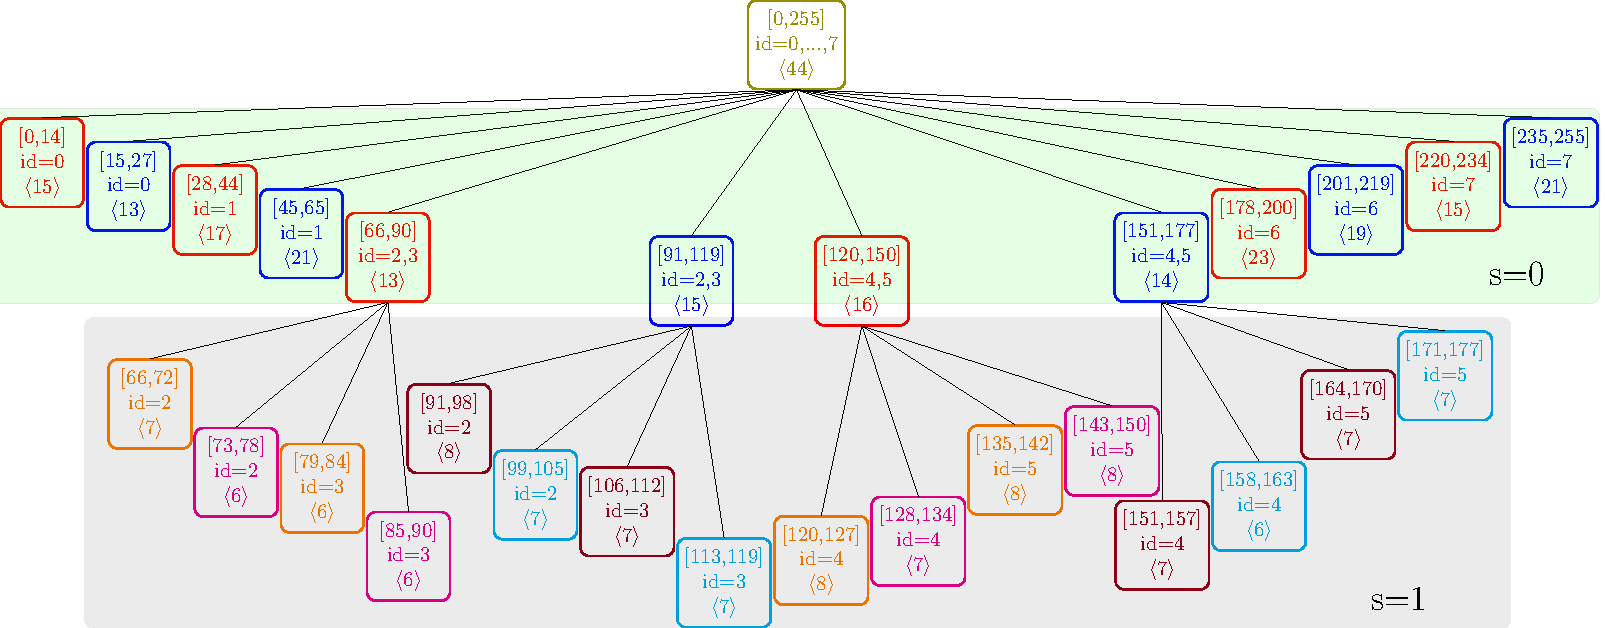
\includegraphics[width=\textwidth, height=0.2\textheight]{pics/recursion/2d-7pt_example/tree/tree}
	 	\caption{The internal tree structure of \acrshort{RACE} representing the \stex for domain size $16 \times 16$ and eight threads. The range $[\ldots]$ specified in each leaf represents the vertices belonging to each \levelGroup and the id refers to the thread id assigned to each \levelGroup assuming compact pinning . The last entry $\langle\acrshort{nrowsEff}\rangle$ gives the effective row number introduced in  \Cref{Sec:param_study}. }
	 	\label{fig:rec_2d-7pt_tree}
	 \end{figure}

\begin{comment}

{\GW Needs to be removed finally from here on till chapter 7}
%
%
%
While we achieved reasonable load balancing for the $16 \times 16$ \stex on five threads in ~\Cref{fig:2d_7pt_lb}, requesting parallelization for eight threads will lead to massive load imbalance due to the \DTWO coloring constraint: At least one thread operating on two inner successive levels has a load of 31 vertices, e.g. if it operates on levels 15 and 16. However, the optimal load per thread is 16 vertices in a single color restricting the parallel speed-up to four, i.e. the parallel efficiency to 50 \%. {\CA This example between 5 and 8 threads is for the necessity of recursion and does not clearly stress the importance of global load balancing. One idea to motivate the importance of global load balancing is by telling currently with recursion we have 2 ways of parallelism one within a stage by increasing level groups of a stage (horizontal parallelism) and second by recursion on a single level group to form level groups in next stage (vertical parallelism). Choosing the right combination of both these parallelism levels require a global load balancing scheme. Current load balancing scheme \Cref{subsec:LB} considers only the horizontal parallelism, now we have to extend it to incorporate also the vertical element of parallelism introduced by recursion.}

Thus, we have to modify/replace  {\GW Christie: can you comment on that (???)} {\CA (It is modification of the existing load balancing step, by allowing more threads per level group)} our original load balancing scheme {\CA{\sout{which assumed a single thread per \levelGroup}}}. {\CA The modification allows multiple threads to be assigned to a single level group $T_{s}(i)$ at stage $s$, threads that are assigned to specific level groups can then be spawned in the subsequent stages ($s+1, s+2, ...$) of recursion. The basic idea here is to assign multiple threads to \levelGroups containing bigger levels, and for simplicity we enforce equal number of threads to adjacent \levelGroups having different color.   To determine the number of threads responsible for a \levelGroup $T_{s}(i)$ following steps are followed:} 

\begin{enumerate}
	\item  First we assign weights to all levels in a specific stage ($s$) of the recursion. Assuming that $L_s(i) \subset T_{s-1}(j)$ its weight is defined by
	
	\begin{align*}
		w(L_s(i)) &= \frac{n_r(L_s(i))}{\frac{\nrowsMath^{total}}{\acrshort{nthreads}^{}}}=\frac{n_r(L_s(i))}{\nrowsMath^{total}}  {\acrshort{nthreads}^{}}\\
		\acrshort{nthreads} &: \text{total number of threads to be used for computing $T_{s-1}(j)$}\\
		\nrowsMath^{total} &= n_r(T_{s-1}(j)) %\text{, i.e. number of vertices in graph}
	\end{align*}
	In the initial stage ($s=0$) the base \levelGroup ($T_{-1}(0)$) is the full matrix/graph and $\acrshort{nthreads}$ is the total number of threads available. This weight describes which fraction of the optimal load per thread ($\frac{\nrowsMath^{total}}{\acrshort{nthreads}^{}}$)  is available in the specific level. 

	For the example shown in \Cref{fig:rec_2d-7pt_graph} requiring 8 threads ($T_{-1}(0) = 8$), weights would be 
	\begin{align*}
		\{w(L_0(0)), w(L_0(1)), w(L_0(2)), ...\} &= \{0.03125, 0.0625, 0.09375, ...\}
	\end{align*}
	
	\item The above definition of weight implies if the weight is close to a natural number $b$, the load induced by rows included in the calculation of weights is close to optimal for operation with $b$ threads. Thus starting with $L_s(0)$ we sum the weights till it forms a number $a$ close to a natural number $b$. Distance-k coloring is ensured by enforcing \atleast $2 \times k$ \levels in the sum, \ie for \DTWO coloring at least four levels (two for red and two for blue) are included. Closeness of the number is measured by a parameter $\epsilon$ defined as:
	\begin{align*}
		\epsilon &=  1 - abs(a-b)\\
		\text{where } b&= \max(1,round(a))
	\end{align*}
	Closeness is controlled by the criteria:
	\begin{align*}
		\epsilon &> \epsilon_s, \text{where $\epsilon_s$ is a control parameter in the range of (0,1)} 	\end{align*}	
	   
	 Once we find a sum satisfying the criteria weight $b$ is fixed. Then we assign first \levelGroup of each color ($T_s(0)$ and $T_s(1)$) to be operated by $b$ threads. With fixed $b$ we try increasing levels in the \levelGroup to check if we can find a better natural number $a'$ closer to $b$ which would increase $\epsilon$ value, if found the new set is considered for allocating weights for $T_s(0)$ and $T_s(1)$. 
	 
	 Thus in case of our example in \Cref{fig:rec_2d-7pt_graph} with $\epsilon_s = 0.6$,  $w(L_0(0)) + w(L_0(1)) + ... + w(L_0(5)) = 0.65625$ satisfies the criteria $\epsilon = 0.65625 > \epsilon_s$, and $b=1$. Therefore one thread ($b=1$) is to be assigned for $T_0(0)$ and  $T_0(1)$. Now fixing $b=1$ we check increasing levels and finally find $w(L_0(0)) + w(L_0(1)) + ... + w(L_0(6)) = 0.875$ gives the highest $\epsilon$ value. Thus for constructing weights of $T_0(0)$ and $T_0(1)$ first 7 levels are used.
	
	\item Weights of subsequent \levelGroups ($T_s(2), T_s(3), ...$) are found by repeating the summing procedure starting with the very next \level. Finally once all the  levels are touched $\acrshort{nthreads}$ threads would be allocated between pairs (red and blue) of \levelGroups. 
	
	For example in case of \Cref{fig:rec_2d-7pt_graph} in order to find number of threads to be assigned for $T_0(2)$ and $T_0(3)$ we start summing from eighth level onwards ($w(L_0(7))$) and find one thread ($b=1$) satisfy the above criteria. For $T_0(4)$ and $T_0(5)$  two threads satisfy the criteria.
\end{enumerate}

Once all the weights are determined using this procedure a weighted load balancing scheme is employed. The scheme remains similar to the one seen in \Cref{subsec:LB} except while calculating mean and variance the weights are considered such that after load balancing ideally a \levelGroup with weight $w$ will have $w$ times more load (rows) than a \levelGroup with weight one. Same algorithm \Cref{alg:LB} presented in \Cref{subsec:LB} can be used except now the weights are the $b$ values instead of ones's. As explained previously in \Cref{subsec:LB} this also takes into account load balancing between different colors (red and blue).

%{\GW Christie: Please describe your scheme step by step with an itemize list and use examples from ~\Cref{fig:rec_2d-7pt_graph}}

    
	\subsubsection{TO BE SKIPPED Internal representation of recursively generated \boldmath{\levelGroups}} \label{subsec:level_tree}
	The recursive nature of our procedure allows to exploit more parallelism. However this introduces more complexity and one has to additionally respect the dependencies between stages and still observe the dependencies within one stage. The best idea is to have a data structure similar to the recursion, therefore we extent the \levelPtr data structure to a hierarchical tree data structure to store these informations. This data structure is called a \levelTree. The root of \levelTree contains information of entire domain, first child leaves of this root \ie leaves with depth 1 stores information about \levelGroups in first stage ($T_0(..)$), leaves with depth 2 stores information about \levelGroups in second stage ($T_1(...)$) and so on. 
	
 
 \Cref{fig:rec_2d-7pt_tree} shows a \levelTree corresponding to \stex  with 8 threads seen in \Cref{fig:rec_2d-7pt_graph}. The leaves in the tree correspond to different \levelGroups and store various informations like the range of vertices or the nodes that belong to this \levelGroup, the effective number of rows (\acrshort{nrowsEff}) that describes the quality of the method (which we will see later in \Cref{Sec:param_study}), and other informations like {\tt thread\_id} assigned to specific \levelGroups.  Threads are assigned to each \levelGroup depending on the pinning strategy used. For example in \emph{fill} type pinning strategy one would pin thread 0 to $T_0(0)$ and $T_0(1)$, thread 1 to $T_0(2)$ and $T_0(3)$, thread 2 to $T_1(0)  \subset T_0(4)$, $T_1(1) \subset T_0(4)$, $T_1(0)  \subset T_0(5)$ and $T_1(1) \subset T_0(5)$, and so on as seen in \Cref{fig:rec_2d-7pt_tree}. 
 
 Note that the \levelTree has a data structure that represents the nested parallelism being used as seen in \Cref{fig:rec_2d-7pt_graph} (right). Therefore threads are spawned based on this \levelTree allowing for easy implementation of point to point synchronizations.

\subsubsection{TO BE SKIPPED Sub-graph selection and global load balancing} \label{subsec:subgraph_selection_old}
Parallelism required for hardware underneath can be obtained either by expanding the \levelTree horizontally \ie increasing \levelGroups within a stage or by expanding \levelTree vertically with the help of recursion. But as we have seen before in \Cref{subsec:DK} the horizontal parallelism is limited by total levels (\acrshort{totalLvl}) and after a certain extent this would lead to load balancing problems. Similarly excessive usage of recursion is also not a good idea since data locality worsens due to local permutations within \subgraph. Therefore it is vital to find a proper balance and choose proper configuration. Furthermore just doing load balancing within a single stage is not the best, for example if we had equally balanced within stage 0 in \Cref{fig:rec_2d-7pt_tree}, we would receive no benefit from recursion. Therefore a global load balancing becomes inevitable.

\Inorder to select proper \subgraph and do global load balancing we employ a simple algorithm to find proper weights for each \levelGroup ($T_s(i)$) in a particular stage, then depending on this weights, denoted as $w(T_s(i))$, we do load balancing with weights in the particular stage $s$ (algorithm for this is similar to \Cref{alg:LB}, except weightage is given to \levelGroups). Finally if $w(T_s(i)) > 1$ we use recursion to achieve $w(T_s(i))$ parallel work in the next stage $T_{s+1}(i)$. The basic structure of the algorithm employed to find weights for the first stage is as follows:
\begin{enumerate}
	\item Find weights, $w(L_0(i))$ for each level in the current stage ($s$) by
		\begin{align*}
			w(L_0(i)) &= (\levelPtr_0[i+1] - \levelPtr_0[i])*\frac{\acrshort{nthreads}}{\nrowsMath^{total}}\\
			\acrshort{nthreads} &: \text{total parallelism required by hardware}\\
			\nrowsMath^{total} &: \text{number of vertices in graph}
		\end{align*}
	
	\item Starting from $w(L_0(0))$ sum up weights till they form a number ($a$) close to whole number ($b$). The closeness can be controlled by an efficiency parameter for stage $s$, $\epsilon_s$ is defined as:
	\begin{equation} \label{eq:epsilon}
		\epsilon_s =  1 - abs(a-b);
	\end{equation}
	All the \levels that are involved in the sum belongs to \levelGroups  operated by first thread in the current stage. The obtained number $b$ is chosen as weight for these \levelGroups \ie $w(T_0(0))=w(T_0(1))=b$. A local search is then done by increasing \levels in this \levelGroups to see if there is a better choice ($a$ close to $b$) with weight $b$, finally \levelGroups are formed with the best choice.  The weight for next \levelGroups are found by resetting the sum counter to zero and repeating the  procedure with \levels just after the current \levelGroups.
\end{enumerate}
For other recursive stage ($s\geq1$) same procedure can be applied to find weights $w(T_s(i))$, except that now $\acrshort{nthreads}$ and $\nrowsMath^{total}$ has to be substituted with the threads required and vertices in the \subgraph considered.

\end{comment}
